%% ---------------------------------------------------------------------------
%%  FEM-6  --  C^1 Bogner-Fox-Schmit framework for fractional-memory
%%             piezoelectric-flexoelectric strain-gradient solids
%%
%%  Layout: elsarticle (3p, times, fleqn); sections and subsections numbered;
%%  figures and tables numbered consecutively; references numbered in citation
%%  order.  The body is split into sec/*.tex and the tables into table_*.tex,
%%  so that a section can be edited without touching the rest.  The figures
%%  are vector PDFs in figures/.
%%
%%  Build: pdflatex -> bibtex -> pdflatex -> pdflatex.  No shell-escape, no
%%  external tool: every package below ships with a standard TeX Live.
%% ---------------------------------------------------------------------------

\documentclass[final,3p,times,fleqn]{elsarticle}

%% ---- packages: all from a standard TeX Live, no shell-escape -------------
\usepackage[T1]{fontenc}
\usepackage[utf8]{inputenc}
\usepackage{graphicx}
\usepackage{amsmath}
\usepackage{bm}
\usepackage{amssymb}
\usepackage{amsthm}
\usepackage{mathrsfs}
\usepackage{mathtools}
\usepackage{multirow}
\usepackage{booktabs}
\usepackage{siunitx}
\usepackage{natbib}
\usepackage{float}
\usepackage[section]{placeins}
\usepackage[colorlinks=true,
            linkcolor=blue,
            urlcolor=blue,
            citecolor=blue]{hyperref}

\biboptions{sort&compress}

%% ---- page layout ----------------------------------------------------------
\parindent 10 pt
\setlength{\topmargin}{-22.0 mm}
\setlength{\headheight}{4.0 mm}
\setlength{\headsep}{10.0 mm}
\setlength{\topskip}{0.00 mm}
\setlength{\textheight}{252.0 mm}
\setlength{\textwidth}{170.0 mm}
\setlength{\oddsidemargin}{-6.0 mm}
\setlength{\evensidemargin}{-3.0 mm}
\linespread{1.0}

\graphicspath{{figures/}}
\journal{Journal name to be supplied}

\begin{document}

\begin{frontmatter}

\title{Fractional-Memory Piezoelectric--Flexoelectric Strain-Gradient Solids
with a Rectangular Nonlocal Window: a $C^1$ Finite Element Framework}

%% TODO  author, affiliation and corresponding e-mail are not supplied in the
%% delivered material; enter them here before submission.
\author{
Author name to be supplied$^{1,*}$
\\
\\
${}^{1}$Affiliation to be supplied\\
Email: $^{1}$address@institution\\
${}^{*}$Corresponding author
}

\begin{abstract}
A $C^1$ Bogner--Fox--Schmit finite element formulation combines
piezoelectricity, flexoelectricity and fractional dielectric memory in a
$\mathrm{BaTiO_3}$ strip. A rectangular averaging window supplies the
gradient stiffness through its second moment, and a Caputo Kelvin--Voigt law
is integrated by the L1 scheme on reduced modal coordinates. Verification uses
closed-form couplings, beam frequencies, gradient identities and the classical
Kelvin--Voigt limit.
The main findings reveal that the extensional coupling factor is
$k^2=0.5581$, within $0.5\,\%$ of the closed form $0.5608$; that rotating an
anisotropic window changes the coupling by $15$--$19\,\%$ while windows of
equal second moment give identical solutions; and that reducing the thickness
of a \SI{200}{\micro\meter}-long strip from \SI{10}{\micro\meter} to
\SI{1}{\micro\meter} multiplies the flexoelectric bending coupling by $24$
while leaving the piezoelectric coupling unchanged to $0.09\,\%$. At
$\alpha=1$ memory on the short-circuit matrix damps $0.450$ times as much as
memory on the condensed one, and the fractional order changes the shape of a
ring-down, not only its decay rate. On a design map of thickness and window
half-thickness the flexoelectric coupling spans $3.6\times10^{-6}$ to
$1.0\times10^{-2}$ and its ratio to the piezoelectric coupling spans
$6.5\times10^{-6}$ to $1.9\times10^{-2}$; the ratio reaches $0.1\,\%$ only
below $h=5.5\,\si{\micro\meter}$ for $a_2=\SI{1}{\micro\meter}$. The assumed
operating range is $a/L\le0.2$. Parameters not supplied by a constitutive
table are stated as assumed inputs. The results support electrode selection,
window and thickness studies, and interpretation of measured ring-downs while
distinguishing geometric size effects from material coupling. Predictions remain
conditional on the stated parameters and memory placement.
\end{abstract}

\begin{keyword}
Flexoelectricity; strain-gradient elasticity; $C^1$ finite elements; nonlocal
averaging window; fractional viscoelasticity; piezoelectric open-circuit sensing
\end{keyword}

\end{frontmatter}

%% ===========================================================================
\FloatBarrier
\section{Introduction}
\label{sec:intro}
%% ===========================================================================

Early device studies show that the electromechanical response of a member a
few micrometers thick is not the response of the same material in bulk. Bending a strip of thickness $h$ to a
curvature $\kappa_c$ produces a strain gradient of order $\kappa_c/h$, so a
coupling that is proportional to the gradient grows as $h^{-2}$ while a coupling
proportional to the strain itself does not; at the micrometer scale the two are
no longer separated by orders of magnitude, and the design of a sensor or a
transducer has to decide which of them it uses. The devices that pose the
question are small and getting smaller: vibration energy harvesters and resonant
microsensors~\cite{Roundy2003,ErturkInman2011}, mechanical metamaterials with
architected microstructure~\cite{Jiao2023}, and additively manufactured parts
whose mesostructure sets a length of its own~\cite{Sarar2024}. These early studies
establish that a device can be designed around a resonant mode of a
millimeter-scale member, measured, and reproduced by a single-length-scale
model; what they leave open is the behavior of the same member when it is
thinner than the mechanism it is built around, which is the regime in which a
gradient coupling and a dielectric memory stop being corrections. Two further
properties of the same devices matter at that scale and are absent from
classical piezoelectricity. The first is that a dielectric driven over decades
of frequency does not respond with a single time constant: its permittivity
follows a broadened dispersion, so the constitutive law is non-local in
time~\cite{ColeCole1941,HavriliakNegami1967}. The second is that the electrodes
are not a detail: whether a polarization is collected depends on which pair of
faces carries the charge, and a formulation that does not distinguish the two
configurations cannot say which effect a measurement is seeing.

Subsequent strain-gradient elasticity supplied the length that the first
property needs, and it did so in a definite order. Toupin~\cite{Toupin1962} proposed a theory of
elastic dielectrics in which the energy depends on the second displacement
gradient, Mindlin and Tiersten~\cite{MindlinTiersten1962} cast the same idea as
a theory of couple stresses, and Mindlin~\cite{Mindlin1964,Mindlin1965} extended
it to a full hierarchy of higher-order elastic constants, first for isotropic
solids and then for crystal classes. Aifantis~\cite{Aifantis1992} proposed to
reduce that hierarchy to a single parameter by keeping only the Laplacian of the
strain in the energy, and Ru and Aifantis~\cite{RuAifantis1993} extended the
reduction to a form that keeps the qualitative predictions of the full theory:
localization is regularized, singularities are removed and stiffness grows as
the member shrinks. In parallel, Eringen and
Edelen~\cite{EringenEdelen1972,Eringen1972Polar,Eringen1983} replaced the local
stress by an integral average over a neighborhood, so the length entered as the
support of a kernel rather than as a coefficient, and Lim~\cite{Lim2015}
combined the two descriptions in a higher-order nonlocal strain-gradient model
in which an integral kernel and a gradient expansion act at once. These
formulations are mathematically complete and geometrically silent: the length is
a constant of the model, and the model cannot say which feature of a
microstructure it stands for. The gap was narrowed from the other side. Reviews
by Askes and Aifantis~\cite{AskesAifantis2011} and
Polizzotto~\cite{Polizzotto2015} compare the formulations, the identification
procedures and the finite element implementations; discrete-to-continuum
arguments show how the gradient terms emerge from a lattice or a representative
volume~\cite{MetrikineAskes2002,Gitman2005}; and homogenization of
three-dimensional lattices establishes that a strain-gradient continuum
reproduces size effects that classical homogenization
misses~\cite{Molavitabrizi2023,YangLiuXia2024}. What none of these routes
delivers is the tensor itself in a form a microscopist could measure: separable
anisotropic gradient models, internal-length tensors and symmetry
classifications of three-dimensional strain-gradient elasticity provide
one~\cite{LazarPo2015,Polizzotto2018,Auffray2019}, but each of them postulates
the tensor and then fits its components to the very test it is meant to predict.
On the criterion of whether the internal length can be measured before it is
used, the averaging domain is the one route that has not been taken.

Later, flexoelectricity supplied the electromechanical side, and its history
is shorter. Kogan~\cite{Kogan1964} identified the coupling of polarization to the
strain gradient, Mindlin~\cite{Mindlin1968} formulated it as a
polarization-gradient theory, Cross~\cite{Cross2006} reviewed its magnitude in
insulating solids, Yudin and Tagantsev~\cite{YudinTagantsev2013} and Zubko and
co-workers~\cite{Zubko2013} reviewed its role in thin films, Codony and
co-workers~\cite{CodonyAriasSuryanarayana2021} computed its transverse component
from first principles for nanostructures at finite deformation, and Lam and
co-workers~\cite{Lam2003} confirmed in micron-scale bending experiments the size
dependence that the gradient predicts. On the computational side the
formulations divide by how they make the second gradient admissible. Mixed and
staggered methods carry it as an independent field and keep $C^0$
interpolation~\cite{AmanatidouAravas2002,AskesMorataAifantis2008,
PhunpengBaiz2015}; micromorphic and virtual element formulations enlarge the
kinematics~\cite{Forest2009,WriggersHudobivnik2023}; Hermite elements carry it
in the interpolation itself~\cite{BognerFoxSchmit1966,PeteraPittman1994,
Zervos2008,Papanicolopulos2009}. Flexoelectric-specific implementations have
followed both routes, with isogeometric analysis for the frequency-domain
response of flexoelectric systems~\cite{ChenYaoYvonnet2023}, computational
homogenization for their topology
optimization~\cite{ChenYvonnetYaoPark2021}, gradient electromechanical finite
elements of arbitrary order~\cite{JoshanSantapuri2024} and a strain-gradient
phase-field formulation for ferroelectrics~\cite{Wang2024PhaseField}; benchmarks
with analytical counterparts~\cite{Yang2021,Lazar2024} and isogeometric
nonlocal-strain-gradient analyses of
nanostructures~\cite{PhungVan2023EC39,PhungVan2024CS335,PhungVan2024TWS198,
Thai2023CS316} complete the landscape. The two routes are not equivalent on the
criterion that decides a coupled calculation, namely how much is spent to make
the gradient admissible: a mixed method adds a symmetric tensor field on every
element and has to stabilize it, whereas a $C^1$ element adds the second
derivatives of the deflection as nodal values and pays in continuity conditions
instead. The mixed route therefore dominates where the geometry is complex and
the mesh must follow it, and the $C^1$ route where the same operator is inverted
many times, as it is when the dielectric law carries a memory and every time
step costs a solve.

Dielectric loss is the third ingredient, and its description predates either
of the other two. A relaxing dielectric is described by a Cole--Cole or a
Havriliak--Negami dispersion~\cite{ColeCole1941,HavriliakNegami1967}, whose
time-domain counterpart is a constitutive law with a memory. Fractional calculus
gives that law one parameter more than elasticity: the spring-pot of
Caputo~\cite{Caputo1967}, used as a constitutive element by Bagley and
Torvik~\cite{BagleyTorvik1983} and by Koeller~\cite{Koeller1984}, reproduces a
power-law relaxation with the order $\alpha$ as the only addition, and it has
been carried into time-domain damping models~\cite{EnelundLesieutre1999} and
into fractional thermo-piezo-elastic wave
problems~\cite{Gupta2026Rayleigh,Gupta2024Impact,Gupta2025Piezo,
Gupta2024Vibrational}. These works establish that one extra order reproduces a
measured dispersion over decades; they leave open what the same order does to
the damping of a device whose stiffness is itself size dependent, because the
element is fitted to a dielectric measurement and then used in a mechanical
time march in which the stiffness is not the bulk one. The cost of that march is
set by where the convolution is carried rather than by the constitutive law: on
the assembled system it grows with the number of degrees of freedom and with
every step, on a small set of modal coordinates it does not, and the price is a
projection that has to be shown to be converged. A modeling decision is usually
left implicit in this literature as well: in a condensed electromechanical
problem two stiffness matrices are available, the condensed one and the
short-circuit one, and a fractional derivative multiplying one is not the same
model as the same derivative multiplying the other.

Taken together, three gaps remain, one for each line. First, the averaging window that gives the
internal length its geometric meaning has not been placed inside a coupled
electromechanical element: the coupled formulations reviewed above use a scalar
length or an assumed tensor, so the relation between the microstructure and the
length that the element sees is not stated. Second, a fractional dielectric
memory has not been formulated in a strain-gradient piezoelectric element with
an explicit statement of which matrix carries the derivative, so the effect of
that choice on a damping ratio is unknown. Third, the coupling factor of a
strain-gradient electromechanical strip has been reported for one electrode
arrangement at a time, without a measure that can be compared across thicknesses
and without separating a material property from a size effect.

Table~\ref{tab:comparison} places the present work against representative
entries from the three lines. Its rows are formulations, not implementations,
and the dashes mark ingredients that the cited paper does not carry; the last
two rows are the one-scale gradient theory of~\cite{fem1} and the present paper.
Read down the window column, the table shows that the geometric length is the
ingredient no coupled formulation carries, and read across the memory column
that the choice of memory matrix is nowhere stated.

%% The comparison table of the introduction.  One row per formulation cited in
%% the text; a dash means the ingredient is not part of that formulation.
\begin{table}[!htbp]
\centering
\small
\caption{Ingredients carried by representative strain-gradient and
flexoelectric formulations. A dash means the ingredient is not part of the
cited formulation; ``splines'' marks $C^1$ isogeometric interpolation. Only
the three last columns distinguish the present work from the one-scale theory
it extends.}
\label{tab:comparison}
\begin{tabular}{@{}lcccccc@{}}
\toprule
formulation & nonlocal or & piezo- & flexo- & frac- & $C^1$ & aniso- \\
 & gradient & electric & electric & tional & & tropic \\
 & & & & memory & & length \\
\midrule
Mindlin, second gradient~\cite{Mindlin1965}          & gradient & -- & -- & -- & -- & -- \\
Eringen, nonlocal elasticity~\cite{Eringen1972Polar} & nonlocal & -- & -- & -- & -- & -- \\
Aifantis~\cite{Aifantis1992}                         & gradient & -- & -- & -- & -- & -- \\
Polizzotto~\cite{Polizzotto2018}                     & gradient & -- & -- & -- & -- & \checkmark \\
Amanatidou and Aravas~\cite{AmanatidouAravas2002}    & gradient & -- & -- & -- & mixed & -- \\
Papanicolopulos and Zervos~\cite{Papanicolopulos2009} & gradient & -- & -- & -- & \checkmark & -- \\
Chen, Yao and Yvonnet~\cite{ChenYaoYvonnet2023}      & gradient & -- & \checkmark & -- & splines & -- \\
Joshan and Santapuri~\cite{JoshanSantapuri2024}      & gradient & -- & \checkmark & -- & -- & -- \\
one-scale theory~\cite{fem1}                         & gradient & -- & -- & -- & \checkmark & \checkmark \\
\textbf{present work} & gradient & \checkmark & \checkmark & \checkmark & \checkmark & \checkmark \\
\bottomrule
\end{tabular}
\end{table}


The novelty lies in three items, one per gap, carried by a single
discretization.

\begin{enumerate}
\item \textbf{A rectangular nonlocal window inside a coupled
  electromechanical element.} The strain-gradient energy is generated by the
  in-plane second-moment tensor $M$ of the averaging window, for which cuboid,
  ellipse and ellipsoid windows give $M_{ii}=a_i^{2}/3$, $a_i^{2}/4$ and
  $a_i^{2}/5$ in closed form. Because the energy is linear in $M$, two windows
  with the same second moment produce identical solutions: the shape of the
  window is not a parameter once $M$ is fixed, whereas its anisotropy and its
  orientation are, and they move the extensional coupling by
  $15$--$19\,\%$.
\item \textbf{Fractional dielectric memory carried on modal coordinates.} The
  dielectric relaxation is a fractional Kelvin--Voigt law of Caputo order
  $\alpha$, discretized by the L1 scheme and convoluted on the reduced modal
  coordinates, which makes the choice of memory matrix an explicit modeling
  decision; at $\alpha=1$ the short-circuit memory damps $0.450$ times as much
  as the condensed one.
\item \textbf{Mode-free coupling factors for two electrode configurations of
  one strip, and the calibration that goes with them.} The coupling factor is
  evaluated from a quasi-static expression that involves no eigenvector, so the
  same measure can be compared across geometries and thicknesses; with it the
  extensional coupling is a material property ($k^{2}=0.5581$, constant to
  $0.09\,\%$ between $10$ and $1\,\mu$m) and the flexoelectric bending coupling
  is a size effect that grows by a factor $24$ over the same range. Each of the
  four model parameters is read from a different observable, and the ranges
  over which the two-dimensional reduction and the small-coupling expansions
  hold are stated.
\end{enumerate}

Section~\ref{sec:formulation} states the formulation and derives the
constitutive relations and the governing equations,
Sec.~\ref{sec:limits} its particular cases, Sec.~\ref{sec:bc} the boundary and
the electrode conditions, and Sec.~\ref{sec:fem} the element, the condensation
and the time stepping. Section~\ref{sec:verification} establishes that the
element solves those equations, Sec.~\ref{sec:results} answers the design
questions, Sec.~\ref{sec:calibration} identifies the parameters and states the
limitations, and Sec.~\ref{sec:conclusions} collects the conclusions.

\FloatBarrier

%% ===========================================================================
\FloatBarrier
\section{Formulation}
\label{sec:formulation}
%% ===========================================================================

The model is a two-dimensional electromechanical continuum with three
enrichments: the strain-gradient energy is generated by the second moment of a
rectangular nonlocal averaging window, the electric enthalpy carries the
piezoelectric and the flexoelectric couplings together, and the dielectric
response is a fractional Kelvin--Voigt law. The derivation below follows the
order in which the finite element needs the result -- window, kinematics,
energy, constitutive relations, reduction, memory, governing equations -- and
the closed-form window coefficients are collected in \ref{app:Mcoeff}.

\FloatBarrier
\subsection{Nonlocal averaging window and the second-moment tensor}
\label{sec:window}

Let the strain gradient at a material point $\bm{x}$ be replaced by its average
over a window $\mathcal{W}$ of area $A_{\mathcal W}$ centred at that point,
\begin{equation}
  \bar\eta_{ijk}(\bm{x}) = \frac{1}{A_{\mathcal W}}
     \int_{\mathcal W} \eta_{ijk}(\bm{x}+\bm{s})\,\mathrm{d}\bm{s}.
  \label{eq:average}
\end{equation}
Expanding the integrand to second order in the window coordinate,
\begin{equation}
  \eta_{ijk}(\bm{x}+\bm{s}) \simeq \eta_{ijk}(\bm{x})
     + s_m\,\eta_{ijk,m}(\bm{x}) + \tfrac12 s_m s_n\,\eta_{ijk,mn}(\bm{x}),
  \label{eq:expand}
\end{equation}
and integrating term by term, the linear term vanishes because the window is
centred, so
\begin{equation}
  \bar\eta_{ijk} \simeq \eta_{ijk} + \tfrac12 M_{mn}\,\eta_{ijk,mn},
  \qquad
  M_{mn} = \frac{1}{A_{\mathcal W}}\int_{\mathcal W} s_m s_n \,\mathrm{d}\bm{s},
  \label{eq:Mdef}
\end{equation}
and every geometric property of the window enters the model through the
symmetric second-order tensor $M$, which has the dimensions of a squared
length and plays the role that a scalar characteristic length plays in
isotropic strain-gradient elasticity. For the three windows used in this work
the diagonal components follow from elementary integration,
\begin{equation}
  M^{\rm cuboid}_{ii} = \frac{a_i^2}{3},\qquad
  M^{\rm ellipse}_{ii} = \frac{a_i^2}{4},\qquad
  M^{\rm ellipsoid}_{ii} = \frac{a_i^2}{5},
  \label{eq:Mshapes}
\end{equation}
where $a_i$ are the half-widths in two dimensions and the semi-axes in three.
A window rotated by $\theta$ in the plane is obtained from the axis-aligned
tensor by $M\mapsto RMR^{\mathsf T}$, that is
\begin{equation}
  M_{11}(\theta)=M_{11}\cos^{2}\theta+M_{22}\sin^{2}\theta,\qquad
  M_{12}(\theta)=\tfrac12\left(M_{22}-M_{11}\right)\sin2\theta,
  \label{eq:Mrot2}
\end{equation}
so the off-diagonal component grows with $\sin2\theta$ and the diagonal ones
carry the orientation dependence.

Equation~\eqref{eq:Mshapes} has a consequence that is used throughout the
paper and is verified in Sec.~\ref{sec:windowshape}: once $M$ is fixed the
\emph{shape} of the window carries no information, because two windows with the
same second moment produce identical solutions. The shape is therefore not a
free parameter of the model, whereas the anisotropy of the window -- its aspect
ratio and its orientation -- is a genuine material-geometry parameter, since it
changes $M$ and with it the ratio between the directional gradient penalties.

\FloatBarrier
\subsection{Kinematics}
\label{sec:kinematics}

Let $\Omega\subset\mathbb{R}^2$ be the mid-plane of a strip of thickness $h$,
with coordinates $x_1$ along the member and $x_2$ through its thickness. The
mechanical state is the pair $(u_1,u_2)$, where $u_1$ is the in-plane
displacement and $u_2\equiv w$ is the transverse deflection, the model retains
the full second gradient of both components, and the strain and the strain
gradient are
\begin{equation}
  \varepsilon_{ij} = \tfrac12\left(u_{i,j}+u_{j,i}\right),\qquad
  \eta_{ijk} = \partial_k \varepsilon_{ij} = \tfrac12\left(
  u_{i,jk}+u_{j,ik}\right),
  \label{eq:strain}
\end{equation}
so that the mechanical degrees of freedom at a node are the eight quantities
\begin{equation}
  \left\{u_1,\; \partial_1u_1,\; \partial_2u_1,\; \partial_{12}u_1,\;
         u_2,\; \partial_1u_2,\; \partial_2u_2,\; \partial_{12}u_2\right\},
  \label{eq:dofs}
\end{equation}
that is, the value, the two first derivatives and the cross derivative of each
component -- eight mechanical degrees of freedom per node and not a
three-component continuum. These are the degrees of freedom of the
Bogner--Fox--Schmit rectangle~\cite{BognerFoxSchmit1966}: a bicubic Hermite
tensor-product element, $C^1$ across element edges and $C^0$ only for the
cross derivative, in which the displacement of one component is interpolated
from its nodal data as
\begin{equation}
  u(\xi,\eta) = \sum_{a=1}^{4}\Big[N^{00}_{a}u_a + N^{10}_{a}u_{,x}\big|_a
    + N^{01}_{a}u_{,y}\big|_a + N^{11}_{a}u_{,xy}\big|_a\Big],
  \label{eq:interp}
\end{equation}
with $N^{pq}_a$ the products of the one-dimensional Hermite cubics. It is the
natural carrier of $\eta_{ijk}$ in two dimensions and it is the element family
used in the one-scale theory~\cite{fem1}; here it is extended by the
flexoelectric and fractional-memory terms rather than replaced.

\FloatBarrier
\subsection{Electric enthalpy and the piezoelectric--flexoelectric
constitutive relations}
\label{sec:energy}

The electromechanical enthalpy of the strip is assembled from five terms. The
elastic energy is
\begin{equation}
  \Pi_{\rm el} = \tfrac12\int_\Omega \varepsilon_{ij} C_{ijkl}
        \varepsilon_{kl}\,\mathrm{d}A ,
  \label{eq:Eel}
\end{equation}
the gradient energy is the window average of the elastic energy truncated at
the second moment, which by \eqref{eq:Mdef} is
\begin{equation}
  \Pi_{\rm gr} = \tfrac14\int_\Omega M_{mn}\,
        \varepsilon_{ij,m}\,C_{ijkl}\,\varepsilon_{kl,n}\,\mathrm{d}A ,
  \label{eq:Egrad}
\end{equation}
the piezoelectric and dielectric energies are
\begin{equation}
  \Pi_{\rm pz} = -\int_\Omega e_{kij} E_k \varepsilon_{ij}\,\mathrm{d}A
  \qquad\text{and}\qquad
  \Pi_{\rm dl} = -\tfrac12\int_\Omega \kappa_{ij} E_i E_j\,\mathrm{d}A ,
  \label{eq:Epiezo}
\end{equation}
and the flexoelectric term is the polarization-gradient coupling of Mindlin's
Form~II~\cite{Mindlin1965,Toupin1962,Mindlin1968},
\begin{equation}
  \Pi_{\rm fx} = -\int_\Omega \mu_{kijl} E_k \eta_{ijl}\,\mathrm{d}A ,
  \label{eq:Eflexo}
\end{equation}
where $E_k=-\phi_{,k}$ is the electric field, $\phi$ the electric potential,
$C_{ijkl}$ the elastic stiffness, $e_{kij}$ the piezoelectric tensor,
$\kappa_{ij}$ the permittivity, $\mu_{kijl}$ the flexoelectric tensor,
$\eta_{ijl}=\varepsilon_{ij,l}$ the strain gradient of \eqref{eq:strain},
$M_{mn}$ the second moment of the averaging window and $W_{\rm ext}$ the work
of the external loads. The total enthalpy is their sum,
\begin{equation}
  \Pi = \Pi_{\rm el} + \Pi_{\rm gr} + \Pi_{\rm pz} + \Pi_{\rm dl}
        + \Pi_{\rm fx} - W_{\rm ext},
  \label{eq:energy}
\end{equation}
in which the isotropic length $\ell^2\delta_{mn}$ of a scalar theory is
replaced by $M_{mn}$ in \eqref{eq:Egrad}. The flexoelectric tensor is taken
isotropic and is represented by the single coefficient
\begin{equation}
  \mu_{kijl} = \mu\,\delta_{ij}\delta_{kl},
  \qquad \mu = 10^{-6}\ \si{\coulomb\per\metre},
  \label{eq:muexplicit}
\end{equation}
a charge per unit length, so every flexoelectric energy in this paper scales as
$\mu$ and every flexoelectric coupling as $\mu^{2}$.

The constitutive relations are the derivatives of $\Pi$ with respect to the
three kinematic variables. The stress is
\begin{equation}
  \sigma_{ij} = \frac{\partial \Pi}{\partial \varepsilon_{ij}}
              = C_{ijkl}\,\varepsilon_{kl} - e_{kij} E_k ,
  \label{eq:sig}
\end{equation}
the higher-order stress is
\begin{equation}
  \varsigma_{ijm} = \frac{\partial \Pi}{\partial \varepsilon_{ij,m}}
              = \tfrac12 M_{mn}\,C_{ijkl}\,\varepsilon_{kl,n}
                - \mu_{kijm}\,E_k ,
  \label{eq:tau}
\end{equation}
and the electric displacement is
\begin{equation}
  D_k = -\frac{\partial \Pi}{\partial E_k}
              = e_{kij}\,\varepsilon_{ij} + \kappa_{kl}\,E_l
                + \mu_{kijl}\,\eta_{ijl},
  \label{eq:D}
\end{equation}
so that the electric displacement contains the strain, the field and the strain
gradient, while the higher-order stress $\varsigma_{ijm}$ is not an
independent constitutive object but the elastic stress transported through the
window. With the single-constant tensor \eqref{eq:muexplicit} the last two
relations become
\begin{equation}
  \varsigma_{ijm} = \tfrac12 M_{mn}\,C_{ijkl}\,\varepsilon_{kl,n}
                    - \mu E_m\delta_{ij},
  \qquad
  D_k = e_{kij}\varepsilon_{ij} + \kappa_{kl}E_l
        + \mu\,\partial_k\left(\varepsilon_{xx}+\varepsilon_{yy}\right),
  \label{eq:Dexplicit}
\end{equation}
which is the form the element assembles. An ellipsoidal window carries
$M_{mn}=L_{mn}/5$ in the notation of the one-scale theory with a tensorial
characteristic length, so $\tfrac14 M_{mn}=\tfrac1{20}L_{mn}$ and the gradient
energy of~\cite{fem1} is recovered exactly.

The three relations are derivatives of the one enthalpy \eqref{eq:energy} taken
with $E_k=-\phi_{,k}$, and their signs are those of the implementation: the
dielectric energy enters $\Pi$ with a minus sign so that $D$ carries
$+\kappa_{kl}E_l$, the assembled dielectric block is
$K_{\phi\phi}=+\int\nabla N_\phi^{\mathsf T}\kappa\nabla N_\phi$, the
piezoelectric coupling is $B=\int B^{\mathsf T}e^{\mathsf T}\nabla N_\phi$, and
the flexoelectric coupling $+\int\mu\,\nabla N_\phi^{\mathsf T}
\nabla(\varepsilon_{xx}+\varepsilon_{yy})$ is carried by the same gradient of
the potential. A sign error in any one of the three would show up as an
asymmetry between $B$ and $B^{\mathsf T}$ rather than as a change of a number.

The second term of \eqref{eq:energy} is the second-moment truncation of the
window average of the elastic energy and not an asymptotic expansion of it:
Taylor expanding the strain about the centroid of the window and averaging
with $\langle s_m\rangle=0$, $\langle s_ms_n\rangle=M_{mn}$ leaves a quadratic
functional in the strain gradient whose kernel is the second-moment tensor, so
the coefficient of the gradient energy is fixed by the window and is not a
fitted length. The truncation is exact for a strain that varies affinely across
the window and is in error at the next order in $a_i\partial\varepsilon$; its
adequacy has to be established for the material at hand
(Sec.~\ref{sec:limit_window}) rather than assumed from a convergent series.

Three remarks on \eqref{eq:energy} matter for the implementation. First, the
gradient term couples the third derivatives of the displacement, so the element
must be $C^1$ in the sense of \eqref{eq:dofs}; a $C^0$ element would make the
fourth-order term non-conforming. Second, the piezoelectric and flexoelectric
couplings appear in the same enthalpy but not in the same devices: they are
collected by different electrode pairs, as Sec.~\ref{sec:bc} makes explicit.
Third, because the strip is treated as a two-dimensional continuum, the
plane-stress or plane-strain reduction of $C$, $e$ and $\kappa$ is part of the
model rather than a detail of the implementation.

\FloatBarrier
\subsection{Two-dimensional reduction of the material tensors}
\label{sec:reduction}

The strip is free out of plane, so the stress component normal to the plane
vanishes and the stiffness that multiplies the in-plane strain is the reduced
tensor
\begin{equation}
  C^{p}_{ij} = C_{ij} - \frac{C_{i3}C_{j3}}{C_{33}},
  \label{eq:Cp}
\end{equation}
with the corresponding reductions of the piezoelectric and dielectric tensors,
\begin{equation}
  e^{p}_{ij} = e_{ij} - \frac{C_{i3}}{C_{33}}\,e_{3j},
  \qquad
  \kappa^{p}_{ij} = \kappa_{ij} + \frac{e_{3i}e_{3j}}{C_{33}},
  \label{eq:ep}
\end{equation}
while the plane-strain alternative keeps $C$ and drops the out-of-plane strain
instead. The two reductions are not interchangeable: for the strip of
Table~\ref{tab:params}, poled along the length, the plane-stress entry is
$C^{p}_{xx}=9.5500\times10^{10}$\,Pa against $C_{xx}=2.22\times10^{11}$\,Pa in
plane strain, and the extensional coupling factor of the two is $0.5581$ and
$0.5132$ respectively. The plane-stress reduction is used everywhere below
because the strip is free out of plane, and the difference between the two is
reported in Sec.~\ref{sec:verification}.

\FloatBarrier
\subsection{Fractional Kelvin--Voigt memory}
\label{sec:fracmem}

The dielectric relaxation is described by a fractional Kelvin--Voigt element in
which the quantity conjugate to the electric field carries a Caputo derivative
of order $\alpha$. The Caputo derivative of a function that starts from rest
is
\begin{equation}
  {}^{C}\!D_t^{\alpha}f(t) = \frac{1}{\Gamma(1-\alpha)}
     \int_{0}^{t}\frac{\dot f(t')}{(t-t')^{\alpha}}\,\mathrm{d}t',
  \qquad 0<\alpha\le1,
  \label{eq:caputo}
\end{equation}
and the spring-pot of Caputo~\cite{Caputo1967}, whose use as a constitutive
element is due to Bagley and Torvik~\cite{BagleyTorvik1983} and
Koeller~\cite{Koeller1984}, is
\begin{equation}
  \sigma(t) = K\,\varepsilon(t) + K\,\tau^{\alpha}\,
              {}^{C}\!D_t^{\alpha}\varepsilon(t),
  \label{eq:kv}
\end{equation}
with $\tau$ a relaxation time and $K$ the appropriate stiffness. The model is
the fractional counterpart of the Cole--Cole description of a broadened
dielectric relaxation~\cite{ColeCole1941,HavriliakNegami1967}, and its
frequency-domain modulus,
\begin{equation}
  K^{*}(\omega) = K\left[1+(\mathrm{i}\omega\tau)^{\alpha}\right],
  \label{eq:kvfreq}
\end{equation}
reduces to the classical Kelvin--Voigt element for $\alpha=1$.

Two matrices are candidates for the $K$ of \eqref{eq:kv} in the condensed
mechanical problem: the fully condensed stiffness $K_{\rm eff}$, which
contains the electrical boundary condition, and the short-circuit stiffness
$K_{uu}$, which does not. They are different models of the same physics, not
two numerical conventions, and Sec.~\ref{sec:memorystudy} quantifies the
difference. Discretising \eqref{eq:caputo} with the L1 scheme at uniform steps
$\Delta t$ gives
\begin{equation}
  {}^{C}\!D_t^{\alpha}\varepsilon(t_n) \approx
  \frac{1}{\Gamma(2-\alpha)}\sum_{k=1}^{n} b_{n-k}\,
  \frac{\varepsilon^{k}-\varepsilon^{k-1}}{\Delta t^{\alpha}},
  \label{eq:l1}
\end{equation}
with the weights
\begin{equation}
  b_j=(j+1)^{1-\alpha}-j^{1-\alpha},\qquad b_0=1,
  \label{eq:bdef}
\end{equation}
computed once for the whole history and reused at every step. Two properties of
the weights are used below: they decay algebraically, so the history is never
forgotten, and at $\alpha=1$ they collapse to $b_0=1$, $b_j=0$ for $j\ge1$, so
that the scheme becomes a backward difference and the memory reduces to the
classical Kelvin--Voigt law up to its first-order truncation error. The
convolution is applied to the reduced modal coordinates, so the history that
has to be stored is one scalar sequence per retained mode and the cost per step
does not grow with the number of elements; which of the two matrices enters
\eqref{eq:kv} decides whether the piezoelectric contribution is inside the
remembered operator or outside it. The L1 discretization is first order in time
for every order $\alpha\in(0,1]$, at $\alpha=1$ as well, because the newest
increment enters through a backward difference; the sequence that measures the
order, and the step the results use, are reported in Sec.~\ref{sec:verification}.

\FloatBarrier
\subsection{Governing equations}
\label{sec:governing}

Stationarity of \eqref{eq:energy} with respect to the mechanical field and to
the potential gives the strong form on $\Omega$,
\begin{align}
  \sigma_{ij,j} - \varsigma_{ijm,jm} + \rho\,\ddot u_i &= 0,
  \label{eq:gov1}\\
  D_{k,k} &= 0,
  \label{eq:gov2}
\end{align}
together with the classical traction and the higher-order double-traction
conditions on the boundary, which are stated in Sec.~\ref{sec:bc}. With
\eqref{eq:Dexplicit} substituted, the two equations read
\begin{equation}
  \left(C_{ijkl}\varepsilon_{kl}\right)_{,j}
    - \left[\tfrac12 M_{mn}C_{ijkl}\varepsilon_{kl,n}\right]_{,jm}
    + \mu\left(\nabla\cdot\bm{E}\right)_{,i} + \rho\ddot u_i = 0,
  \qquad
  \kappa_{kl}E_{l,k} = -\mu\,\partial_k\partial_k
    \left(\varepsilon_{xx}+\varepsilon_{yy}\right),
  \label{eq:govexp}
\end{equation}
so that \eqref{eq:gov1} carries the flexoelectric term
$\mu(\nabla\cdot\bm E)_{,i}$ and \eqref{eq:gov2} carries
$\mu\partial_k\partial_k(\varepsilon_{xx}+\varepsilon_{yy})$; the two are the
transpose pair that the weak form assembles. The mechanical boundary condition
of the gradient theory is the pair $(t_i,\,m_i)$ -- force and double force per
unit length -- so a clamped edge constrains both the displacement and its
normal derivative, exactly the quantities that appear in \eqref{eq:dofs}. In
the time domain the memory of \eqref{eq:kv} turns \eqref{eq:gov1} into a
Volterra-type equation whose kernel is the fractional derivative of
\eqref{eq:l1}; the weak form of Sec.~\ref{sec:fem} is written directly for the
time-discrete problem, which is what the implementation solves.

Three effects enter at this point and are kept apart throughout: the memory of
\eqref{eq:kv} acts on the \emph{damping} at fixed eigenfrequency, the window of
\eqref{eq:Mdef} acts on the \emph{stiffness} at fixed memory, and the
flexoelectric tensor $\mu$ acts on the \emph{coupling} at fixed geometry. No
result below is attributed to one of them when it was computed with another
changed.

The two electrode arrangements referred to throughout the paper are fixed in
Fig.~\ref{fig:geometry}: the bending family is poled across the thickness with
electrodes on the long faces, and the extensional family is poled along the
length with electrodes on the end faces. They are two electrical
configurations of one strip, and the coupling factors obtained from them are
therefore not additive.

The parameters of the model are collected in Table~\ref{tab:params}. The
elastic, piezoelectric and dielectric constants are the values measured by
Zgonik and co-workers for $\mathrm{BaTiO_3}$~\cite{Zgonik1994}; the mass
density is the standard crystallographic value for the same material. Five
quantities are assumed rather than measured, and they are listed in the same
table: the flexoelectric coefficient, taken as
$\mu=10^{-6}$\,\si{\coulomb\per\metre}, which is the order reported for
perovskite ceramics, so that every flexoelectric coupling below is to be read
as scaling with $\mu^{2}$; the window half-widths, which are held at
$a_1/L\le0.2$ as the operating range of the second-moment truncation assumes;
the fractional order and the relaxation time, which are free parameters of the
memory law and are varied over the ranges stated; and the mesh, which the
convergence study of Sec.~\ref{sec:verification} shows to be adequate for
every quantity quoted.

%% The parameter table: quantity, symbol, value, unit.  The source of every
%% value is stated in the sentence above the table, not in a column.
\begin{table}[!t]
\centering
\small
\caption{Parameters of the model. The sources of the first four rows are given
in the text above the table; the five rows below the rule are assumed and their
effect is stated there and in Secs.~\ref{sec:material} and
\ref{sec:limitations}.}
\label{tab:params}
\begin{tabular}{@{}llll@{}}
\toprule
quantity & symbol & value & unit \\
\midrule
elastic constants & $C_{11}$, $C_{12}$, $C_{13}$, $C_{33}$, $C_{44}$ &
$222$, $108$, $111$, $151$, $61$ & GPa \\
piezoelectric constants & $e_{15}$, $e_{31}$, $e_{33}$ &
$34.2$, $-0.7$, $6.7$ & \si{\coulomb\per\square\metre} \\
relative permittivities & $\kappa_{11}/\kappa_0$, $\kappa_{33}/\kappa_0$ &
$2200$, $56$ & -- \\
mass density & $\rho$ & $6020$ & \si{\kilo\gram\per\cubic\metre} \\
\midrule
flexoelectric coefficient & $\mu$ & $10^{-6}$ & \si{\coulomb\per\metre} \\
window half-widths & $a_1$, $a_2$ & $3$, $1$ & \si{\micro\metre} \\
fractional order & $\alpha$ & $0.5$--$1$ & -- \\
relaxation time & $\tau$ & $0.3$--$30$ & \si{\nano\second} \\
strip geometry & $L$, $h$ & $200$, $10$ & \si{\micro\metre} \\
mesh & -- & $48\times4$ BFS elements & -- \\
\bottomrule
\end{tabular}
\end{table}


\begin{figure}[!t]
\centering
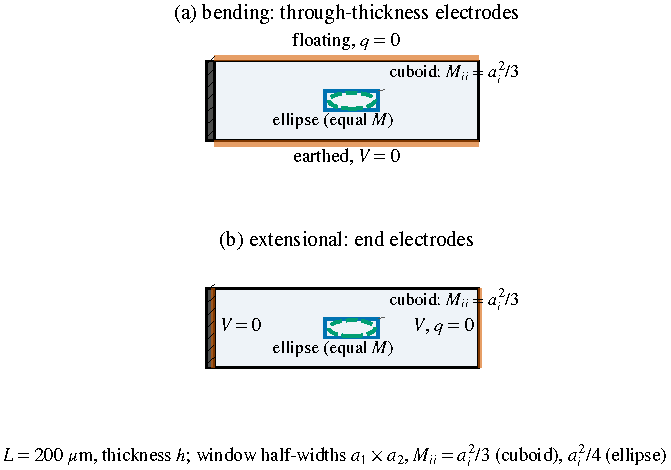
\includegraphics[width=\textwidth]{F1_geometry.pdf}
\caption{The two electrode configurations and the averaging window.
(a) Bending family, poled through the thickness: electrodes on the large
faces, the lower earthed and the upper floating at zero net charge.
(b) Extensional family, poled along the length: electrodes on the short ends.
The window is a rectangle of half-widths $a_1\times a_2$, whose second moment
fixes the gradient energy.}
\label{fig:geometry}
\end{figure}

\FloatBarrier

%% ===========================================================================
\FloatBarrier
\section{Particular cases}
\label{sec:limits}
%% ===========================================================================

The general model of Sec.~\ref{sec:formulation} contains four switches, and
each of them has to reproduce a known theory when it is turned off. This
section states those reductions; the numerical results that follow are read
against them, and Sec.~\ref{sec:verification} checks two of them as exact
identities rather than as trends.

\FloatBarrier
\subsection{Classical piezoelectricity: $M_{mn}\to0$ and $\mu_{kijl}\to0$}
\label{sec:limit_classical}

If the averaging window shrinks to a point, $M_{mn}\to0$, the gradient energy
in \eqref{eq:energy} vanishes. That alone does not remove the higher-order
stress: by \eqref{eq:tau} it reduces to $-\mu_{kijm}E_k$, so a model with a
window of zero size and a nonzero flexoelectric coefficient keeps a
higher-order stress, a double traction and a fourth-order character. Classical
piezoelectricity is therefore the double limit $M_{mn}\to0$ \emph{and}
$\mu_{kijl}\to0$, in which the double-traction condition of Sec.~\ref{sec:bc}
drops out of the formulation. What remains is the classical piezoelectric strip: the weak
form keeps only the elastic, piezoelectric and dielectric terms, the
displacement field needs $C^0$ continuity only, and the coupling factor is the
purely piezoelectric one. The window size is therefore the single parameter
that switches the model from a local electromechanical theory to a
strain-gradient one, and it does so without changing any other term.

\FloatBarrier
\subsection{Purely piezoelectric response: $\mu_{kijl}=0$}
\label{sec:limit_piezo}

With the flexoelectric tensor set to zero the electric displacement
\eqref{eq:D} loses its strain-gradient contribution and the model reduces to
the linear piezoelectric strip of the plane-stress reduction
\eqref{eq:Cp}, with the strain-gradient stiffness retained. On the extensional configuration of
Fig.~\ref{fig:geometry} the coupling factor is $k^2=0.5581$ and is unchanged by
the switch, because that configuration collects the piezoelectric charge only.
On the bending configuration the piezoelectric charge of the mode integrates
to zero over a face electrode, and the piezoelectric-only coupling factor of
that mode falls to $1.0\times10^{-10}$, which is the round-off floor of the
secular equation rather than a physical value. The comparison of the two
configurations therefore cannot be read as a competition between the two
effects; it is a statement about which electrode pair can collect which
polarization.

\FloatBarrier
\subsection{Purely flexoelectric response: $e_{kij}=0$}
\label{sec:limit_flexo}

Removing the piezoelectric coupling instead leaves the flexoelectric bending
response of the same strip. Over the thickness range
$\SI{10}{\micro\metre}\to\SI{1}{\micro\metre}$ the flexoelectric coupling of
that configuration then rises from $1.76\times10^{-4}$ to
$5.5\times10^{-3}$, a factor $31$. With the piezoelectric terms present the
same sweep gives a rise from $1.74\times10^{-4}$ to $4.2\times10^{-3}$, a
factor $24$. The piezoelectric terms are electrically silent on that device,
but they are not mechanically silent: they change the elastic stiffness of the
mode that carries the gradient, and the difference between $24$ and $31$ is
the measure of that change. Both are reported, and the paper quotes the factor
$24$ because it is the response of the real crystal.

\FloatBarrier
\subsection{Classical Kelvin--Voigt and undamped limits: $\alpha=1$ and
$\tau\to0$}
\label{sec:limit_memory}

For $\alpha=1$ the fractional element \eqref{eq:kvfreq} becomes the classical
Kelvin--Voigt element, whose exact damping ratio is $\omega\tau/2$. The
implementation reproduces it: at $\omega\tau=0.3$ the ring-down of
Sec.~\ref{sec:memorystudy} returns $\zeta_{\rm eff}=0.15003$ against the exact
$0.15000$, a difference of $0.02\,\%$. For $\tau\to0$ the memory term of
\eqref{eq:kv} vanishes, the time-discrete problem \eqref{eq:step} becomes the
undamped one, and the eigenvalues of the pencil are those of the short-circuit
matrix. Between these two limits the model is genuinely fractional: the
damping ratio is no longer proportional to $\omega\tau$, and the memory matrix
that the derivative multiplies changes $\zeta_{\rm eff}$ by a factor $0.450$
at $\alpha=1$ (Sec.~\ref{sec:memorystudy}).

\FloatBarrier
\subsection{Recovery of the one-scale gradient theory}
\label{sec:limit_fem1}

Finally, the one-scale gradient theories are recovered as special choices of
$M$. For an ellipsoidal window $M_{mn}=L_{mn}/5$, so
$\tfrac14M_{mn}=\tfrac1{20}L_{mn}$ and the tensorial strain-gradient energy of
the one-scale theory~\cite{fem1} is reproduced exactly, with the cuboid,
ellipse and ellipsoid windows giving the scalar coefficients that
\ref{app:Mcoeff} lists; setting $M_{mn}=\ell^{2}\delta_{mn}$ reduces the same
expression to the isotropic Aifantis form~\cite{Aifantis1992}. Dropping the
memory and the flexoelectric tensor leaves the classical piezoelectric strip.
The present work differs from these in carrying the fractional memory on the
reduced modal coordinates and in treating the window's second moment, rather
than a scalar length, as the object that the discretization sees.

\FloatBarrier

%% ===========================================================================
\FloatBarrier
\section{Boundary conditions}
\label{sec:bc}
%% ===========================================================================

The fourth-order character of \eqref{eq:gov1} means that a boundary condition
on the displacement is not enough: the gradient theory requires a second,
higher-order condition on each edge, and the electrical condition decides
which of the two coupling factors the model returns. This section fixes both,
together with the axes that the rest of the paper refers to.

\FloatBarrier
\subsection{Mechanical and higher-order conditions}
\label{sec:bc_mech}

On an edge with unit outward normal $\bm{n}$ and tangent $\bm{t}$, stationarity
of \eqref{eq:energy} gives the classical traction
\begin{equation}
  t_i = \sigma_{ij}n_j - \partial_m\!\left(\varsigma_{ijm}\right)n_j
      + \partial_t\!\left(\varsigma_{ijm}\,t_m n_j\right),
  \label{eq:traction}
\end{equation}
and the higher-order double traction
\begin{equation}
  m_i = \varsigma_{ijm}\,n_j n_m ,
  \label{eq:doubletraction}
\end{equation}
which is conjugate to the normal derivative of the displacement. Three
combinations are used in the results:

\begin{enumerate}
\item \emph{clamped}: $u_i=0$ and $u_{i,j}n_j=0$ on the edge, so that both the
  displacement and its normal derivative -- the two quantities carried by the
  element \eqref{eq:dofs} -- are prescribed;
\item \emph{simply supported}: $u_i=0$ together with $m_i=0$, which leaves the
  slope free and removes the double force;
\item \emph{free}: $t_i=0$ and $m_i=0$, the natural conditions of the weak
  form, which are satisfied automatically by the discretization.
\end{enumerate}

The clamped condition is the one that produces the boundary layer of a
gradient theory: the gradient energy penalises the curvature that the
prescribed slope forces at the edge, so the solution relaxes over a length set
by the window. Section~\ref{sec:windowshape} measures that layer against
$a/L$, and the results are consistent with the ratio $a/L\le0.2$ that the
paper adopts as its validity window.

\FloatBarrier
\subsection{Electrical conditions: open and short circuit}
\label{sec:bc_elec}

Two electrical conditions are used. In the \emph{short-circuit} configuration
the electrode pair is grounded, the internal potential degrees of freedom are
condensed, and the mechanical problem has stiffness $K_{sc}$. In the
\emph{open-circuit} configuration one electrode is grounded and the other
floats at a single potential $V$ carrying zero net charge, which is again a
condensation and gives the rank-one update
\begin{equation}
  K_{oc} = K_{sc} + \frac{1}{\beta}\, d\,d^{\mathsf T},
  \label{eq:rankone}
\end{equation}
with $d$ the condensed coupling vector and $\beta$ the condensed dielectric
coefficient. Two coupling measures follow from this pair, and the difference
between them matters for the interpretation of every coupling number in the
paper:
\begin{enumerate}
\item the \emph{mode-based} factor of the $j$-th mode,
  $k_j^2=(\omega_{oc,j}^2-\omega_{sc,j}^2)/\omega_{oc,j}^2$, which depends on
  the eigenvector that the solver happened to return;
\item the \emph{mode-free quasi-static} factor of the electrode pair,
  \begin{equation}
    x = \frac{d^{\mathsf T}K_{uu}^{-1}d}{\beta},\qquad
    k^2 = \frac{x}{1+x},
    \label{eq:kstatic}
  \end{equation}
  which involves no eigenvector at all.
\end{enumerate}
Equation~\eqref{eq:kstatic} is the measure used wherever a quantity has to be
compared across geometries or across thicknesses, because it cannot select a
different mode in a different configuration. Four symbols carry the distinction
in what follows and are fixed here once: $k^2_{\rm qs}=x/(1+x)$ is the
mode-free factor of \eqref{eq:kstatic}; $k^2_{\rm qs,u}=x$ is the same
quantity without the coupled denominator, the one that can be set against
$e^{\mathsf T}C^{-1}e/\kappa$; $k^2_{j}$ is the mode-based factor of the
$j$-th mode; and $k^2_{j}(K_{uu})$ or $k^2_{j}(K_{sc})$ names the matrix whose
short-circuit eigenvalues enter it. An unsubscripted $k^2$ in the results is
$k^2_{\rm qs}$. The extensional coupling factor
of the \SI{200}{\micro\metre} by \SI{10}{\micro\metre} plate obtained from
\eqref{eq:kstatic} is $k^2=0.5581$, within $0.5\,\%$ of the constitutive
prediction $0.5608$ obtained from the constitutive tensors in
Sec.~\ref{sec:verification}.

\FloatBarrier
\subsection{Poling axes and Voigt indices}
\label{sec:axes}

The material is tetragonal $\mathrm{BaTiO_3}$ at room temperature, and the
crystal is anisotropic, so the two configurations of Fig.~\ref{fig:geometry}
do not share a modulus: poling along $x$ pairs the strain $\varepsilon_{xx}$
with $C^p_{xx}=9.5500\times10^{10}$\,Pa, while poling along $y$ pairs the same
strain with $C^p_{xx}=1.6946\times10^{11}$\,Pa, the two being exchanged by the
rotation that takes one poling axis into the other. Table~\ref{tab:axes} fixes
the axes, the Voigt indices and the tensors once, so that every later formula
can be read against it; a modulus may only be paired with the permittivity of
its own configuration, and the wrong pairing is examined, and excluded, in
Sec.~\ref{sec:verification}.

\begin{table}[!htbp]
\centering
\small
\caption{Which axis, which Voigt index, which modulus. (a) The axes of the
model: Voigt indices are $1=x$, $2=y$, $3=z$ throughout, and $z$ is a basal
direction of the $4mm$ crystal in both orientations. (b) The two
configurations used in the paper. They share the geometry and the material
record but not the poling axis, and a modulus may only be paired with the
permittivity of its own configuration.}
\label{tab:axes}
% table generated from the archived results
\begin{tabular}{@{}llll@{}}
\toprule
\multicolumn{4}{@{}l}{\emph{(a) the model axes, Voigt indices $1=x$, $2=y$, $3=z$}}\\
axis & role & extent & what it carries\\
\midrule
$x$ & length & \SI{200}{\micro\metre} & bending: $\varepsilon_{xx}=\kappa y$; the piezoelectric load direction\\
$y$ & thickness & \SI{10}{\micro\metre} & strain gradient $\partial\varepsilon_{xx}/\partial y=\kappa$; the flexoelectric gap\\
$z$ & out of plane & -- & neutral axis of the bending (curvature about $z$), free surface\\
\midrule
\multicolumn{4}{@{}l}{\emph{(b) the two configurations; they differ in the poling axis, and therefore in which entry of $\bm C_p$ multiplies $\varepsilon_{xx}$}}\\
& & piezo $k^2$ (\ref{sec:verification}) & flexo check (\ref{app:verification})\\
\midrule
poling axis & & $x$ & $y$\\
electrodes & & $x=0$, $x=L$ (short faces) & $y=0$, $y=h$ (long faces)\\
gap & & $L=$\SI{200}{\micro\metre} & $h=$\SI{10}{\micro\metre}\\
permittivity across the gap & & $\kappa_{xx}=\kappa_{33}=$\SI{4.9583e-10}{\farad\per\metre} & $\kappa_{yy}=\kappa_{33}=$\SI{4.9583e-10}{\farad\per\metre}\\
$C^p_{xx}$ & multiplies $\varepsilon_{xx}$ & \SI{9.5500e10}{\pascal} & \SI{1.6946e11}{\pascal}\\
$C^p_{yy}$ & & \SI{1.6946e11}{\pascal} & \SI{9.5500e10}{\pascal}\\
$E_b=1/(\bm C_p^{-1})_{xx}$ & beam modulus & \SI{7.6327e10}{\pascal} & \SI{1.3544e11}{\pascal}\\
coupling & & $\bm e_p^{\mathsf T}\bm C_p^{-1}\bm e_p/\kappa_{xx}$ & $3\mu^2/(C^p_{xx}h^2\kappa_{yy})$\\
\bottomrule
\end{tabular}

\end{table}

The pairing rule has a quantitative consequence that the paper relies on. The
extensional configuration is poled along $x$ with electrodes on the short
faces and the gap $L=\SI{200}{\micro\metre}$; the bending configuration is
poled along $y$ with electrodes on the long faces and the gap
$h=\SI{10}{\micro\metre}$. The two gaps differ by a factor of twenty, and so do
the electric fields produced by the same polarization, which is why the
extensional coupling is an electromechanical property of the material and the
bending coupling is a size effect of the geometry.

\FloatBarrier

%% ===========================================================================
\FloatBarrier
\section{Finite element formulation}
\label{sec:fem}
%% ===========================================================================

\FloatBarrier
\subsection{Weak form}
\label{sec:weak}

Testing \eqref{eq:gov1} and \eqref{eq:gov2} against a virtual displacement
$\delta\bm{u}$ and a virtual potential $\delta\phi$ and integrating by parts
twice, the strain-gradient term produces both the double traction
\eqref{eq:doubletraction} and an integral over the element interiors,
\begin{multline}
  \int_\Omega \delta\varepsilon_{ij}\,C_{ijkl}\,\varepsilon_{kl}\,\mathrm{d}A
  + \tfrac12\int_\Omega \delta\varepsilon_{ij,m}\,M_{mn}\,C_{ijkl}\,
     \varepsilon_{kl,n}\,\mathrm{d}A \\
  - \int_\Omega \delta\varepsilon_{ij}\,e_{kij}\,E_k\,\mathrm{d}A
  - \int_\Omega \delta\varepsilon_{ij,m}\,\mu_{kijm}\,E_k\,\mathrm{d}A \\
  - \int_\Omega \delta E_k\left(e_{kij}\varepsilon_{ij}
     + \kappa_{kl}E_l + \mu_{kijl}\eta_{ijl}\right)\mathrm{d}A
  = \delta W_{\rm ext}
  + \int_{\Gamma}\left(\delta u_i\,t_i + \delta u_{i,j}n_j\,m_i\right)
    \mathrm{d}s ,
  \label{eq:weak}
\end{multline}
which is the form that the element matrices implement. The boundary integral
carries the two mechanical conditions of Sec.~\ref{sec:bc_mech}; the electrical
term carries the electrode conditions of Sec.~\ref{sec:bc_elec} and is
condensed before assembly, so that the mechanical problem never sees the
potential degrees of freedom.

\FloatBarrier
\subsection{The BFS element and its degrees of freedom}
\label{sec:bfs}

The domain is covered by Bogner--Fox--Schmit rectangles. Each element has four
nodes and, per node, the eight mechanical degrees of freedom \eqref{eq:dofs}
carried by a bicubic Hermite tensor-product interpolation, that is 32
mechanical degrees of freedom per element, together with the four nodal
potentials of a bilinear interpolation. The strain and the strain gradient on
the element are
\begin{equation}
  \varepsilon = B(\xi,\eta)\,\bm{u}^e,\qquad
  \eta_k = \partial_k\varepsilon = B_{,k}(\xi,\eta)\,\bm{u}^e,
  \label{eq:Bmat}
\end{equation}
both integrated by $2\times2$ Gauss quadrature in the element frame; the
gradient matrix $B_{,k}$ contains the third derivatives of the shape functions
and is the reason the element has to be $C^1$. The element contributions are
the elastic $K_e=\int B^{\mathsf T}CB$, the gradient
$K_{g,e}=\tfrac12\int M_{mn}B_{,m}^{\mathsf T}CB_{,n}$, the piezoelectric coupling
$B_e=\int B^{\mathsf T}e^{\mathsf T}\nabla N_\phi$, the dielectric
$C_{\phi,e}=-\int\kappa\,\nabla N_\phi\cdot\nabla N_\phi$ and a consistent mass
matrix from the same interpolation. The flexoelectric contribution is
assembled into $B_e$ as the additional potential--displacement coupling that
the $\mu_{kijl}\eta_{ijl}$ term of \eqref{eq:energy} produces; because it
involves $B_{,k}$, it is the term for which the $C^1$ character of the element
is indispensable.

\FloatBarrier
\subsection{Condensation of the potential}
\label{sec:condensation}

The assembled system is indefinite in the saddle-point form
\begin{equation}
  \begin{bmatrix} K & B \\ B^{\mathsf T} & -C_\phi \end{bmatrix}
  \begin{bmatrix} \bm{u} \\ \bm{\phi}\end{bmatrix}
  = \begin{bmatrix} \bm{f} \\ \bm{q}\end{bmatrix},
  \label{eq:saddle}
\end{equation}
with $C_\phi$ positive by construction. Eliminating the potential degrees of
freedom of the electrode set reproduces \eqref{eq:rankone} exactly, and the
returned pair $(d,\beta)$ is what the modal and the static solvers consume.
Two conventions are enforced in the implementation because they are easy to get
wrong: the charge is read as $q=d^{\mathsf T}\bm{u}/\beta$ rather than by
pointwise integration of the electric displacement, and eigenvectors are
phase-normalized on a nodal displacement degree of freedom -- normalizing on
$\max|\phi|$ can select a derivative degree of freedom and return a
meaningless voltage.

\FloatBarrier
\subsection{Modal L1 time stepping}
\label{sec:stepping}

With the L1 weights of \eqref{eq:l1} the time-discrete problem is
\begin{equation}
  \left(M + \Delta t^{\alpha}\Gamma(2-\alpha)\,K_{\rm mem}\right)\bm{a}^n
  = \bm{f}^n - K\bm{u}^n - K_{\rm mem}\sum_{k=1}^{n-1} b_{n-k}
    \left(\bm{u}^{k}-\bm{u}^{k-1}\right),
  \label{eq:step}
\end{equation}
solved by a Cholesky factorization of the constant left-hand matrix, with
$K_{\rm mem}\in\{K_{\rm eff},K_{uu}\}$ the model choice quantified in
Sec.~\ref{sec:memorystudy}. In the modal variant used for the long ring-downs,
the same convolution is carried on the mass-normalized coordinates of the
retained modes, so the cost per step is proportional to the number of retained
modes rather than to the number of degrees of freedom; the truncation error of
that projection is measured against the full-order solution rather than
assumed small (Sec.~\ref{sec:verification}).

\FloatBarrier
\subsection{Implementation remarks}
\label{sec:implementation}

Two properties of the implementation are worth recording, because they
govern both cost and accuracy.

\begin{enumerate}
\item \emph{Scaling.} The gradient block is $O(M/h^4)$ while the elastic block
  is $O(C/h)$, so the assembled pencil becomes badly scaled as the thickness
  falls. The implementation scales the two blocks separately before the
  eigensolve and returns the eigenpairs unscaled; the thin-plate limit of
  Sec.~\ref{sec:thickness} is at a condition number of about $10^{12}$, and the
  sensitivity of the resulting small differences is measured rather than
  assumed (\ref{app:verification}).
\item \emph{Cost.} A mesh of $48\times4$ BFS elements has $49\times5=245$
  nodes and $8\times245=1960$ mechanical degrees of freedom and is the
  workhorse of the results; the mesh-refinement study of
  Sec.~\ref{sec:verification} shows that on that mesh the frequency of the
  extensional mode is within $0.05\,\%$ and its quasi-static coupling factor
  within $0.03\,\%$ of a $96\times4$ refinement, and the thinnest plates are
  solved on it because the conditioning, not the number of elements, is the
  binding constraint.
\end{enumerate}

\FloatBarrier

%% ===========================================================================
\FloatBarrier
\section{Validation and limiting cases}
\label{sec:verification}
%% ===========================================================================

\FloatBarrier
\subsection{Material, geometry and discretization}
\label{sec:material}

The parameters that the four cases of this section share are fixed once here,
so that each case varies only the feature it is meant to test; the material is
tetragonal $\mathrm{BaTiO_3}$ at room temperature, with the constants of
Table~\ref{tab:params}.

The dielectric anisotropy ratio
$\kappa_{11}/\kappa_{33}=39$ is retained, so the two poling configurations
differ in their permittivity as well as in their modulus. The strain-gradient
length scale is set by the window: with half-widths
$a_1\times a_2=3\times1$\,\si{\micro\meter} the cuboid window of
\eqref{eq:Mshapes} gives $M_{11}=3.0\times10^{-12}$ and
$M_{22}=3.3\times10^{-13}$\,\si{\square\meter}, that is characteristic lengths
$\sqrt{M_{11}}=\SI{1.73}{\micro\meter}$ and
$\sqrt{M_{22}}=\SI{0.58}{\micro\meter}$ along and across the strip. The ratio
$a_1/L=0.015$ is far inside the assumed operating range $a/L\le0.2$ of
Sec.~\ref{sec:limit_window}, using the inputs of Sec.~\ref{sec:formulation}.
The density $\rho$ rescales every frequency by the common factor
$1/2\pi\sqrt{\rho}$ and therefore moves the kilohertz numbers without touching
any ratio. The flexoelectric coefficient $\mu$ enters every
flexoelectric energy linearly and every flexoelectric coupling as $\mu^{2}$,
so the growth factors and the comparison with the piezoelectric response stand
whatever its value, while the absolute flexoelectric coupling follows it
quadratically.

\FloatBarrier
\subsection{Case I: benchmarks and mesh convergence}

The first case asks whether the element reproduces answers that are known
independently of it, and at what mesh the answers stop moving; the full record
of benchmarks, identities and independent routes is \ref{app:verification}.
In every case the solver assembles the weak form \eqref{eq:weak} with the
Hermite interpolation \eqref{eq:interp}, applies the kinematic conditions
\eqref{eq:bcmech}, and returns the higher-order stress \eqref{eq:sig} from the
constitutive relations of \eqref{eq:govexp}.

Three problems with known answers were solved with the same element: a
one-dimensional strain-gradient bar, whose static tip displacement and
frequency were compared with the closed form; the same bar in the classical
limit; and the constant-strain patch test. The clamped-free and clamped-clamped
frequencies of the strip agree with the Euler--Bernoulli values to $0.26\,\%$
and $0.10\,\%$, and the elastic strip reproduces the gradient theory whenever
the window is set to zero. Figure~\ref{fig:convergence} then shows the error in
the frequency of the extensional mode and in its quasi-static coupling factor
against the number of degrees of freedom. Both converge from above at the rate
expected of a bicubic Hermite interpolation, and the $48\times4$ mesh used
throughout the paper is inside the asymptotic range: refining it to $96\times4$
changes the frequency by $0.05\,\%$ and the coupling factor by $0.03\,\%$,
while the coarser $24\times2$ mesh used for the parameter sweeps differs from
it by $0.04\,\%$ and $0.03\,\%$. Table~\ref{tab:convergence} lists the four
meshes.

\begin{figure}[!htbp]
\centering
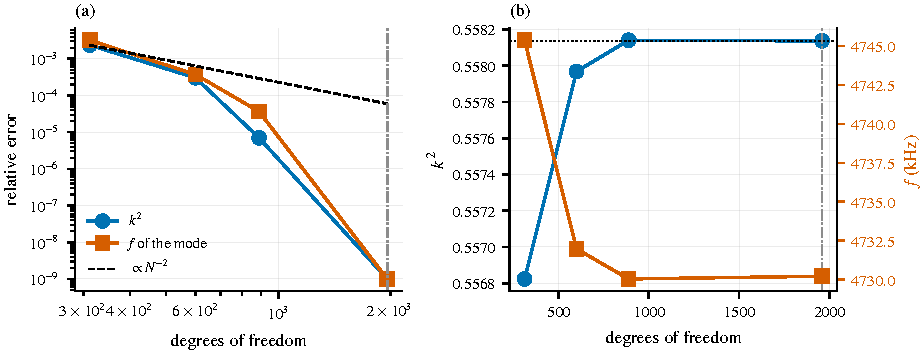
\includegraphics[width=\textwidth]{F2_convergence.pdf}
\caption{Variations of (a) the relative error of the extensional coupling factor $k^2$ and of the frequency of the mode that carries it, both referred to the finest mesh, and of (b) the two quantities themselves, against the number of mechanical degrees of freedom. The line in (a) is the $N^{-2}$ rate of a bicubic Hermite interpolation, the dotted line in (b) the converged value, and the $48\times4$ mesh is marked. The strip uses the material and geometry of Table~\ref{tab:params}, poling along $x$, plane stress and zero window size.}
\label{fig:convergence}
\end{figure}

\subsection{Case II: the coupling factor and its closed form}

The second case asks whether the assembled model reproduces the constitutive
coupling factor, which is the one quantity here that can be obtained without a
mesh.

The coupling factor of the extensional electrode pair is the one quantity in
this paper that can be obtained without a mesh, and doing so fixes the meaning
of every assembled value that follows. From the constitutive tensors alone,
\begin{equation}
  x=\frac{e^{\mathsf T}C_{p}^{-1}e}{\kappa}=1.2768,
  \qquad
  k^{2}=\frac{x}{1+x}=0.5608 ,
  \label{eq:xclosed}
\end{equation}
which is the closed-form value for the plane-stress strip; the
three-dimensional free bar gives $0.5771$, the three-dimensional uniaxial case
$0.3748$ and the two-dimensional plane-strain case $0.5132$, all from the same
tensors and all listed in \ref{app:data}. The plane-stress value is
the relevant one, because the strip is free out of plane.

The assembled model returns three numbers that belong to this same closed
form and differ from it for stated reasons. With the window switched off and
the strip unconstrained, the assembled route reproduces \eqref{eq:xclosed} to
$1.2\times10^{-11}$ relative, at $0.56079$: that is the validation of the
assembly, a comparison of two computations of one number. Clamping the left edge lowers the coupling to $0.55957$,
because the clamp restrains the in-plane deformation that carries the
piezoelectric charge, and switching the window on lowers it further to
$0.55814$, because the gradient stiffness adds energy to the same mode without
adding charge. The working value quoted in the abstract is the last of the
three, $k^{2}=0.5581$, which is $0.4\,\%$ below the free-strip closed form and
is the value a clamped device actually has. The two mode-based values,
$k^2_4=0.4650$ on the elastic memory matrix and $k^2_4=0.4583$ on the
short-circuit stiffness, are different measures again and are introduced where
the ring-down uses them (Sec.~\ref{sec:memorystudy}); they are not comparable
with the mode-free ones and are never averaged with them.

\subsection{Case III: time discretization and the step used}

The third case asks whether the L1 march converges at the order the scheme
promises and which step the ring-downs later use.

The L1 scheme is first order in $\Delta t$ for every $\alpha\in(0,1]$, at
$\alpha=1$ as well. At $\alpha=1$ and $\omega\tau=0.3$ the damping ratio
extracted from the ring-down is $0.150111$, $0.150057$ and $0.150029$ at $N$,
$2N$ and $4N$ steps over twenty periods ($N=12000$, that is $600$ steps per
period), against the exact $\omega\tau/2=0.150000$: halving the step halves the
residual, an observed order of $0.97$, and the sequence extrapolates to the
exact value. The ring-downs of Sec.~\ref{sec:memorystudy} are run at the $4N$
step. The eight curves of Sec.~\ref{sec:transient} are a coarser march, $400$
steps per period, and their decrements carry the step in the last decimal.

\subsection{Case IV: the fields of the coupled bending mode}

The fourth case asks whether the coupled solution has the spatial structure
the constitutive model implies: a bending mode that is electrically silent in
the piezoelectric sense, and a through-thickness strain gradient that is not.

Figure~\ref{fig:fields} records the four fields of the coupled bending mode in
the open-circuit configuration, together with the strain gradient that drives
the flexoelectric term. The in-plane and the transverse displacement are those
of a first bending mode; the potential is not. It reaches tens of millivolts a
few tens of micrometers from the clamped edge and near mid-height, and falls
toward both the edge and the free end, so the two face electrodes sit where the
potential is smallest. That is the spatial form of the cancellation that makes
this configuration insensitive to the piezoelectric charge and responsive to
the strain gradient, and the gradient panel shows where the flexoelectric
charge is generated: in the boundary layer at the clamp and along the neutral
axis, not at the electrodes.

\begin{figure}[!htbp]
\centering
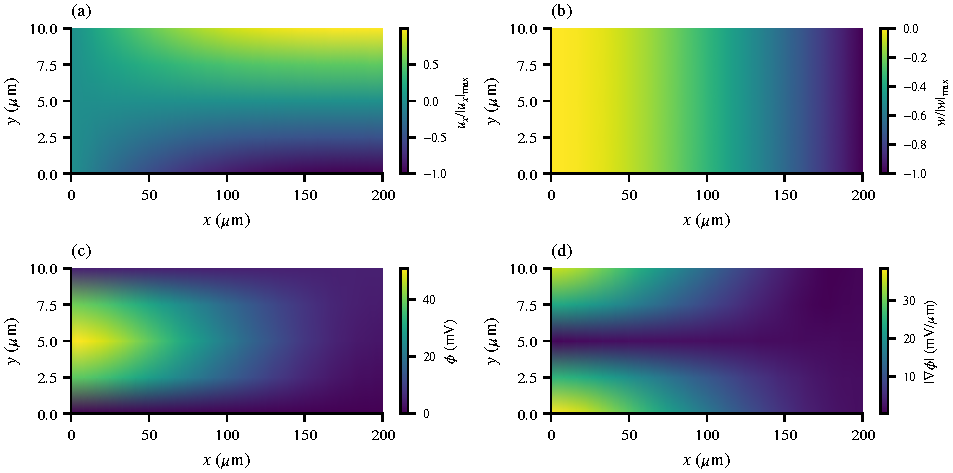
\includegraphics[width=\textwidth]{F3_fields.pdf}
\caption{Variations of (a) the in-plane displacement, (b) the deflection, (c) the potential at \SI{10}{\nano\meter} of tip motion, (d) the electric field and (e) the magnitude of the strain gradient that drives the flexoelectric term over the coupled bending mode, in the open-circuit configuration on a $48\times4$ mesh, with the geometry, material and window of Table~\ref{tab:params}, poling along $y$ and plane stress. The potential is smallest at the face electrodes and the gradient largest at the clamp.}
\label{fig:fields}
\end{figure}

\FloatBarrier
\subsection{The worked calculation of the headline numbers}
\label{sec:worked}

The numbers quoted in the abstract follow from the inputs in four short steps,
collected here so that the route from a material constant to a coupling factor
is visible and not only its outcome; Table~\ref{tab:worked} lists inputs and
outputs side by side.

\paragraph{Window} For half-widths $a_1=\SI{3}{\micro\meter}$ and
$a_2=\SI{1}{\micro\meter}$ the second-moment tensor of the cuboid window is
diagonal with
\begin{equation}
  M_{11}=\frac{a_1^{2}}{3}=3.000\times10^{-12}\ \si{\meter\squared},\qquad
  M_{22}=\frac{a_2^{2}}{3}=3.333\times10^{-13}\ \si{\meter\squared},
  \label{eq:Mnumber}
\end{equation}
an anisotropy ratio $M_{11}/M_{22}=9$. The three shapes are interchangeable
once $M$ is fixed, because $M_{ii}=a_i^{2}/3$, $a_i^{2}/4$ and $a_i^{2}/5$ for
the cuboid, the ellipse and the ellipsoid: an ellipsoid of half-width
$a_{\rm ell}=1.2910\,a_{\rm cub}=\sqrt{5/3}\,a_{\rm cub}$ reproduces
\eqref{eq:Mnumber} exactly, and the reciprocal
$a_{\rm cub}=0.7746\,a_{\rm ell}$ is the conversion used for the equal-$M$ pair
of Sec.~\ref{sec:windowshape}.

\paragraph{Plane-stress reduction and closed form} The strip is free out of
plane, so the stiffness that multiplies $\varepsilon_{xx}$ is the reduced entry
\eqref{eq:Cp}, which for $\mathrm{BaTiO_3}$ gives
$C^{p}_{xx}=9.5500\times10^{10}$\,Pa with the poling along $x$ and
$1.6946\times10^{11}$\,Pa with the poling along $y$, and
$C^{p}_{12}=5.7000\times10^{10}$\,Pa in both cases. The entries that pair with
it are $e_{33}=6.7$ and $e_{31}=-0.7$\,\si{\coulomb\per\square\meter} and the
permittivity across the electrode gap,
$\kappa_{yy}=\kappa_{33}=4.9583\times10^{-10}$\,\si{\farad\per\meter}. Hence
$x=1.2768$ and $k^{2}=0.5608$ from \eqref{eq:xclosed}, with no mesh involved.

\paragraph{Assembled route} The same quantity on the assembled model comes from
one short-circuit and one open-circuit reduction of the $48\times4$ mesh:
$245$ nodes, eight mechanical degrees of freedom per node ($1960$ unknowns)
and $245$ potential unknowns, condensed to a single electrode pair $(d,\beta)$
with $\beta=2.4792\times10^{-11}$\,\si{\farad}. Then
\begin{equation}
  x_{\rm FEM}=\frac{d^{\mathsf T}K_{sc}^{-1}d}{\beta}=1.2631,
  \qquad
  k^{2}_{\rm FEM}=\frac{x_{\rm FEM}}{1+x_{\rm FEM}}=0.5581 ,
  \label{eq:xFEM}
\end{equation}
$0.47\,\%$ below \eqref{eq:xclosed}; the clamped edge accounts for $0.22\,\%$
of that and the gradient stiffness for a further $0.26\,\%$.

\paragraph{Flexoelectric smallness and L1 weights} With the piezoelectric
constants switched off, the same reduction gives the smallness parameter of the
bending configuration,
\begin{equation}
  x=\frac{3\mu^{2}}{C^{p}_{xx}\,h^{2}\,\kappa_{33}}
   =\frac{3\,(10^{-6})^{2}}{1.6946\times10^{11}\cdot(10^{-6})^{2}\cdot
     4.9583\times10^{-10}}
   =3.5704\times10^{-4}
  \label{eq:xflexo}
\end{equation}
at $h=\SI{10}{\micro\meter}$, against a finite element value of
$1.7437\times10^{-4}$; the two routes differ by a factor $2.05$ and the
difference is discussed with the thickness sweep in Sec.~\ref{sec:thickness}.
The L1 weights are fixed numbers that do not depend on the model,
\begin{equation}
  \alpha=0.5:\; (b_0,b_1,b_2)=(1,\;0.414214,\;0.317837),\qquad
  \alpha=0.7:\; (b_0,b_1,b_2)=(1,\;0.231144,\;0.159245),
  \label{eq:bweights}
\end{equation}
and the damping ratio follows from the decrement of two successive peaks,
\begin{equation}
  \delta=\ln\frac{A_k}{A_{k+1}},\qquad
  \zeta_{\rm eff}=\frac{\delta}{\sqrt{4\pi^{2}+\delta^{2}}} ,
  \label{eq:zeta}
\end{equation}
of which $\zeta=\delta/2\pi$ is the small-damping approximation. At
$\omega\tau=0.3$ the ratio of two successive voltage peaks is $2.5947$, so
$\delta=0.95345$ and $\zeta_{\rm eff}=0.15003$ against the exact
$\omega\tau/2=0.15000$.

%% Summary of the worked calculation: inputs -> intermediate -> output.
\begin{table}[!htbp]
\centering
\small
\caption{The headline numbers of the abstract, from their inputs. Each value
is the one carried into the figures and tables of this section; the last column
is the number the abstract quotes.}
\label{tab:worked}
\begin{tabular}{@{}p{0.20\textwidth}p{0.22\textwidth}p{0.24\textwidth}p{0.24\textwidth}@{}}
\toprule
quantity & inputs & intermediate & value \\
\midrule
extensional coupling & $C_p$, $e$, $\kappa_{33}$ &
$x=1.2768$; $x_{\rm FEM}=1.2631$ & $0.5581$ ($0.5608$ closed form) \\
thickness independence & $k^2$ at $10$ and \SI{1}{\micro\meter} &
$0.55814\to0.55861$ & $0.09\,\%$ \\
flexoelectric growth & $\mu$, $C^{p}_{xx}$, $h$, $\kappa_{33}$ &
$1.7437\times10^{-4}\to4.1736\times10^{-3}$ & factor $24$ \\
flexoelectric slope & the eight thicknesses & local log--log slopes &
$-1.96$ to $-0.43$ \\
window anisotropy & $M_{11}$, $M_{22}$, $\theta$ & $M$ rotates, the mesh does
not & $15$--$19\,\%$ \\
two configurations & \eqref{eq:xclosed} in both & $0.4580$ against $0.1141$;
\SI{138.99}{\volt} against \SI{2.41}{\volt} & factor $58$ \\
memory ratio & $K_{\rm eff}$, $K_{uu}$ & $\zeta=0.15003$ against $0.06746$ &
$0.450$ \\
integer-order limit & $\omega\tau=0.3$ & $\zeta_{\rm eff}$ against
$\omega\tau/2$ & $0.02\,\%$ \\
\bottomrule
\end{tabular}
\end{table}


The four cases and the worked calculation fix the input set of the paper: the
material constants of Table~\ref{tab:params}, the window of
Sec.~\ref{sec:material} and the mesh sizes named above. With them the
quantities of Sec.~\ref{sec:results} follow, and each of those results is
reported below as a figure, a mechanism and a number.

\FloatBarrier

%% ===========================================================================
\FloatBarrier
\section{Numerical results and discussion}
\label{sec:results}
%% ===========================================================================

The five design questions raised in Sec.~\ref{sec:intro} are answered here, one
subsection each: whether the direction in which the microstructure is sampled
matters, what the size and the shape of the window do, whether thinning a device
helps, what the memory order and the relaxation time do to the damping, and what
the four electrode configurations return for one strip. Every number quoted is a
solved eigenvalue or a time march of the model of Sec.~\ref{sec:formulation},
discretized as in Sec.~\ref{sec:fem} and checked as in
Sec.~\ref{sec:verification}. The inputs are those of Sec.~\ref{sec:formulation}; the worked calculation
is in Sec.~\ref{sec:worked} and the tables in \ref{app:data} and
\ref{app:verification}.

\FloatBarrier
\subsection{Window orientation and window aspect ratio}
\label{sec:orientation}

Figure~\ref{fig:orientation} shows what the orientation of an anisotropic
sampling window is worth, which is the first design question because the
gradient energy is linear in the second-moment tensor $M$ and a rotation of the
window changes $M$ without changing the strip. The window is held at a
half-width of \SI{3}{\micro\meter} along its long axis; its aspect ratio is
${\rm AR}=a_1/a_2$. The strip is
\SI{200}{\micro\meter}$\times$\SI{10}{\micro\meter}, for the poling-$x$
configuration that carries the response; physically, the window is the domain
over which the microstructure of the film is averaged, so its orientation
decides which component of the strain gradient the material is asked to
transmit. Over the $6\times19$ cuboid cases the extensional mode remains the one
with the largest coupling, its short-circuit frequency varying smoothly from
$4907$ to \SI{5296}{kHz}, so the mode identity is not in question while the
window turns.

\subsubsection{Why one quadrant is computed}

The strip maps onto itself under $\theta\to\theta+180^\circ$. The second
invariance is a symmetry of the whole problem and not of the energy alone: the
gradient energy is \emph{linear} in $M$, so a change of sign of $M_{12}$ by
itself changes the response, and what leaves it unchanged is the reflection
$y\to-y$, which maps $\theta\to-\theta$ and at the same time maps the strip,
the electrode pair and -- for poling along $x$, the configuration plotted here
-- the material onto themselves. The response is therefore even in $\theta$ for
the poling-$x$ configuration; for poling along $y$ the same reflection reverses
the poling direction and is not a symmetry of the material, so only the period
$180^\circ$ holds and the orientation study is confined to poling $x$. Neither
invariance is assumed: both are evaluated at \SI{15}{\degree} intervals for the
extreme aspect ratios, where they reproduce the computed points to
$3\times10^{-11}$ relative.

\subsubsection{What the orientation is worth}

The extensional frequency and coupling move monotonically with $\theta$ and saturate by
$\theta=90^\circ$. The extensional frequency rises from $5012$ to
\SI{5296}{kHz} at ${\rm AR}=2$ and from $4907$ to \SI{5288}{kHz} at
${\rm AR}=10$, that is by $6$--$8\,\%$, while the coupling falls from $0.4448$
to $0.3786$ and from $0.4677$ to $0.3801$ between the same two orientations, a
change of $15$--$19\,\%$. The fundamental mode of the same strip, which carries
a coupling three orders of magnitude smaller, moves from \SI{146.4}{kHz} to
\SI{158.1}{kHz} at ${\rm AR}=10$. At $\theta=0^\circ$ the window aspect ratio is
worth $0.4448\to0.4677$ between ${\rm AR}=2$ and ${\rm AR}=10$, about
$5\,\%$, and the aspect ratios collapse onto $0.3786$--$0.3801$ at
$\theta=90^\circ$: once the long axis of the window is transverse to the strain
gradient, its aspect ratio no longer matters.

The coupling plotted here is the \emph{total} coupling of the extensional mode
and it is piezoelectric in the main; the flexoelectric contribution at
$\mu=10^{-6}$\,\si{\coulomb\per\meter} is of order $10^{-4}$
(Sec.~\ref{sec:thickness}), so the window acts on the modal coupling through
the gradient stiffness rather than by adding a flexoelectric term directly.
Figure~\ref{fig:design} separates the two. Panel (a) is the change of the
coupling against the aligned window: largest for the most elongated window,
$-18.7\,\%$ at ${\rm AR}=10$ and $\theta=90^\circ$, and weakest for the
squarest, $-14.9\,\%$ at ${\rm AR}=2$. Panel (b) is
$(M_{11}-M_{22})/(M_{11}+M_{22})$, shown for ${\rm AR}=2$, which
passes through zero at $45^\circ$ and changes fastest there. The coupling
follows the anisotropy of the second-moment tensor and not the shape of the
window. Hence the orientation of the window is a design variable worth
$15$--$19\,\%$ of the coupling, while the aspect ratio of an already elongated
window is worth $5\,\%$ or less once the window is turned transverse to the
gradient.

\begin{figure}[!htbp]
\centering
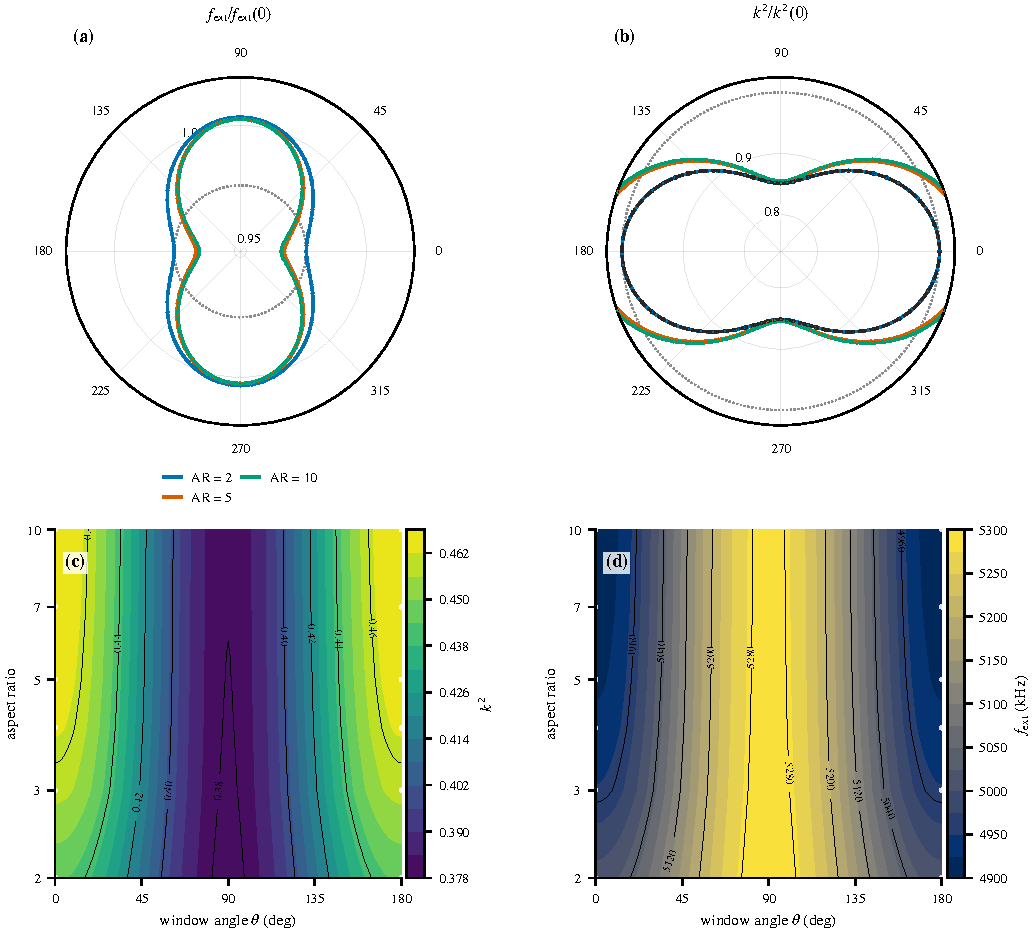
\includegraphics[width=\textwidth]{F4_orientation.pdf}
\caption{Variations of (a) the extensional frequency and (b) its coupling factor, both normalized to the aligned ${\rm AR}=2$ window, over the full circle of window orientation, and of (c) the coupling factor and (d) the frequency as maps over orientation and window aspect ratio, for a \SI{200}{\micro\meter}$\times$\SI{10}{\micro\meter} strip with poling along $x$, plane stress and a $24\times2$ mesh. Markers are computed points, lines a periodic spline. The long window half-width is \SI{3}{\micro\meter}.}
\label{fig:orientation}
\end{figure}

\begin{figure}[!htbp]
\centering
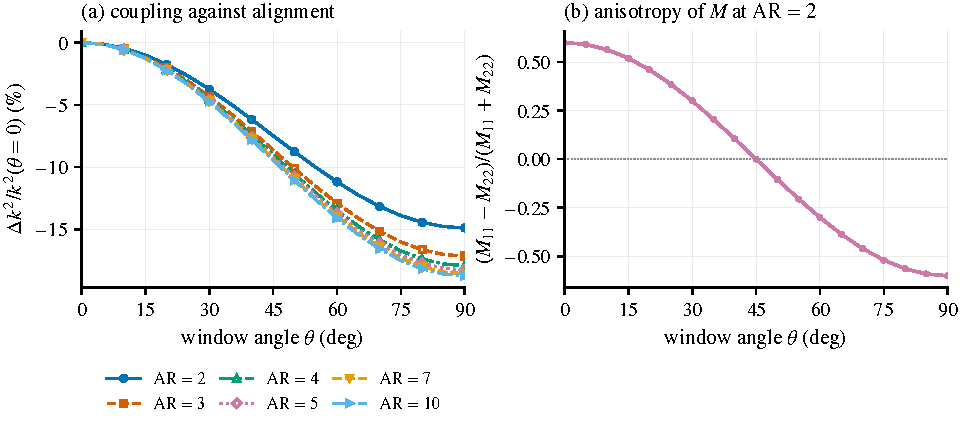
\includegraphics[width=0.86\textwidth]{F5_design.pdf}
\caption{Variations of (a) the change of the extensional coupling relative to the aligned window, one curve per window aspect ratio, and of (b) the anisotropy of the second-moment tensor at ${\rm AR}=2$, for the window and poling of Fig.~\ref{fig:orientation}. The coupling spans $4$ percentage points at $90^\circ$ and reaches $-18.7\,\%$ where the anisotropy of (b) is largest.}
\label{fig:design}
\end{figure}

\FloatBarrier
\subsection{Memory order, relaxation time and the damping map}
\label{sec:memorystudy}

Figure~\ref{fig:damping} shows how the two parameters of the dielectric law move
the damping of a mode, and the answer separates into a modeling and an
implementation question. The modeling question is the fractional
Kelvin--Voigt element of \eqref{eq:kv}, which differs measurably from the
integer-order element that finite element codes usually provide; physically,
$\alpha$ measures how broad the relaxation spectrum is, a single time constant
at $\alpha=1$ and a spectrum spread over decades below it, while $\tau$ is the
center of that spectrum and fixes the $\omega\tau$ at which the loss peaks. The
implementation question is the convolution of \eqref{eq:step}, which may
multiply the fully condensed stiffness $K_{\rm eff}$ or only the short-circuit
matrix $K_{uu}$; the two give different damping, and the difference is not a
numerical detail. The loss tangent \eqref{eq:tandelta} and its small-loss limit
\eqref{eq:zetasmall} of Sec.~\ref{sec:calib_alpha_tau} are what the map plots,
and the integer-order limit it is compared against is \eqref{eq:limitKV}.

\subsubsection{Which matrix carries the memory}

Table~\ref{tab:memory} reports the ring-down of the extensional mode (mode 4,
\SI{6.727}{MHz}) at $\tau=\SI{7.0974}{\nano\second}$, that is $\omega\tau=0.3$,
with an initial tip displacement that produces \SI{139.07}{\volt} of
open-circuit voltage at $t=0$. Three coupling numbers for that mode appear in
the paper and they come from two quantities:
$k^2_{4}(K_{uu})=0.4650$ is the mode-based measure on the elastic memory matrix
$K_{uu}$ and $k^2_{4}(K_{sc})=0.4583$ is the same measure on the short-circuit
stiffness $K_{sc}$, both on the $24\times2$ mesh of the ring-down; the third,
$0.4580$ in Sec.~\ref{sec:application}, is $k^2_{4}(K_{sc})$ again,
recomputed with $\mu=0$ because that section quotes the material without
flexoelectricity. The gap of $1.5\,\%$ between $0.4650$ and $0.4583$ reflects the
choice of short-circuit stiffness in the coupling measure, while the
$0.07\,\%$ between $0.4583$ and $0.4580$ reflects the inclusion of $\mu$.

The damping ratio is extracted from two successive peaks with
\eqref{eq:zeta}. At the $\omega\tau=0.3$ of Table~\ref{tab:memory} the ratio of
two successive voltage peaks is $2.5947$, so $\delta=0.95345$ and
$\zeta_{\rm eff}=0.15003$ for $K_{\rm eff}$ at $\alpha=1$, against the exact
$\omega\tau/2=0.15000$: the implementation reproduces the classical limit to
$0.02\,\%$. Refining the step gives $\zeta_{\rm eff}=0.150111$, $0.150057$ and
$0.150029$ at $N$, $2N$ and $4N$ steps over twenty periods, so the residual is
first order in $\Delta t$ (observed order $0.97$) and extrapolates to
$0.150000$; every ring-down quoted in this section is run at the $4N$ step.
Replacing $K_{\rm eff}$ by $K_{uu}$ removes the piezoelectric contribution from
the memory and takes the ratio $\zeta(K_{uu})/\zeta(K_{\rm eff})$ at $\alpha=1$
down to $0.450$, so the short-circuit memory dissipates $55\,\%$ less. The
difference is of the order of the coupling ($k^2_{4}=0.4650$) but does
\emph{not} reduce to the naive factor $1-k^2=0.535$: the two memories differ by
the piezoelectric stiffness that the condensation puts into $K_{\rm eff}$, and
its effect on the ring-down has to be computed rather than estimated. For a
strongly piezoelectric device the distinction belongs in the model statement,
not in the implementation.

Neither matrix is derived from a dielectric relaxation; both are placements of
the fractional element inside a condensed model. One law can be derived
exactly. If the permittivity itself relaxes,
$D_k=e_{kij}\varepsilon_{ij}+\kappa_{kl}[1+(\tau\partial_t)^{\alpha}]E_l$,
then $\nabla\cdot\bm D=0$ carries the Caputo derivative of the field, and
condensing the potential moves the memory onto the piezoelectric stiffening
$B_iC^{-1}B_i^{\mathsf T}$, that is onto exactly the part of $K_{\rm eff}$ that
the condensation adds over $K_{uu}$. That is a third possibility, bracketed by
the two matrices tabulated: $K_{\rm eff}$ remembers the whole condensed
stiffness and $K_{uu}$ none of it. The ratio $0.450$ belongs to the
$\alpha=1$ row of Table~\ref{tab:memory} and to this device.

%% The memory-matrix comparison, moved from the appendix to the text.
\begin{table}[!htbp]
\centering
\small
\caption{Ring-down with the memory carried on the condensed stiffness
$K_{\rm eff}$ and on the short-circuit stiffness $K_{uu}$ (mode 4,
\SI{6.727}{MHz}, $\omega\tau=0.3$). At $\alpha=1$ the entry is the damping
ratio \eqref{eq:zeta}; at $\alpha=0.7$ the decay is not exponential and the
entry is the first-period decrement.}
\label{tab:memory}
\begin{tabular}{@{}lcc@{}}
\toprule
memory matrix & $\alpha=1$: $\zeta_{\rm eff}$ &
  $\alpha=0.7$: first-period $\zeta$ \\
\midrule
$K_{\rm eff}$ & $0.15003$ & $0.1942$ \\
$K_{uu}$      & $0.06746$ & $0.0831$ \\
\midrule
ratio $K_{uu}/K_{\rm eff}$ & $0.450$ & $0.428$ \\
\bottomrule
\end{tabular}
\end{table}


\subsubsection{Decay at fractional order}

At $\alpha=0.7$ the free decay is not exponential and a single damping ratio
does not exist: the successive decrements of the $K_{\rm eff}$ ring-down are
$1.244$, $1.547$, $0.010$, $0.403$, $0.240$ and $0.151$; the first, second,
fourth, fifth and sixth of them are unchanged to three digits between
$\Delta t$, $\Delta t/2$ and $\Delta t/4$, so they are a property of the
fractional element -- whose relaxation is a Mittag-Leffler function, not an
exponential -- and not of the step, while the third is a near-cancellation
between two peaks of comparable height. A straight line fitted to $\ln A_k$, with $A_k$ the successive peak amplitudes,
over the twenty periods therefore returns a number that is not a damping ratio,
which is why the $\alpha=0.7$ column of Table~\ref{tab:memory} carries the
first-period decrement rather than a fitted slope. The $\alpha=1$ entries are
unaffected: there the twenty successive decrements agree to $7\times10^{-10}$
relative, which is why \eqref{eq:zeta} applies.

\subsubsection{Fractional against integer-order element}

The fractional element differs from the integer-order one by more than
accuracy; it differs in shape. At the device point $\omega\tau=0.3$ the
Kelvin--Voigt model over-predicts the modulus by $3.5\,\%$ at $\alpha=1$ and by
$22.6\,\%$ at $\alpha=0.7$; at $\omega\tau=1$ the ratio of the two is $1.35$
and $1.62$, and at $\omega\tau=100$ the integer-order model is wrong by a
factor $91$. A single-relaxation fit is unusable outside the narrow band where
it was fitted, which is the band a design map is meant to cover.

\subsubsection{The damping map}

Figure~\ref{fig:damping}(a) is the pole of \eqref{eq:kvfreq} in the complex
plane, traced over $\omega\tau$ for seven relaxation times and colored by
$\tau$, with markers at five Caputo orders; Fig.~\ref{fig:damping}(b) is the
damping ratio $\zeta=-\mathrm{Re}\,s/|s|$, where $s$ is the dimensional
complex pole and $\omega_0$ the undamped angular frequency, over the
$(\alpha,\omega\tau)$ plane. Both are computed with branch continuation: the
root is followed from one $\omega\tau$ to the next by initializing the Newton
iteration at the adjacent converged pole, without which the iteration jumps to a spurious
root of the negative-real-part branch. All poles lie in the left half-plane for
every $(\alpha,\tau)$ examined, so the fractional Kelvin--Voigt element is
dissipative by construction. The integer-order case sits at
$|\mathrm{Im}\,s|/\omega_0\simeq1$ for $\omega\tau\lesssim0.1$ and moves down
and to the right as $\omega\tau$ grows, so the dashpot lowers the frequency and
eventually over-damps the mode: at $\omega\tau=10$ the imaginary part has
vanished and $\zeta=1$. The fractional cases fan \emph{upward}: a spring-pot
with $\alpha<1$ raises the damped frequency as $\tau$ grows, because the
fractional modulus grows sub-linearly rather than linearly in $\omega$. At
$\omega\tau=10$ and $\alpha=0.5$ the damped frequency is $2.13\,\omega_0$
($2.45\,\omega_0$ at $\alpha=0.7$), against $\mathrm{Im}\,s=0$ for $\alpha=1$ at
the same $\omega\tau$. The ratio in Fig.~\ref{fig:damping}(b) increases with
both $\alpha$ and $\omega\tau$ and reaches $\zeta\to1$ for $\alpha\to1$ and
large $\omega\tau$; for small $\alpha$ it is flat, because a spring-pot with a
broad relaxation spectrum produces a damping that depends only weakly on the
device frequency. That flatness is the qualitative reason the fractional
description is used for dielectric loss in the first place. The band
$\omega\tau\le1$, which contains the strip mode at \SI{6.73}{MHz} for every
$\tau\le\SI{32}{\nano\second}$ used here, is the one in which the element is
calibrated and claimed. Hence, in the range where the element is used, $\alpha$
sets the shape of the decay and $\tau$ sets where the loss peaks, and neither of
them alone fixes a damping ratio.

\begin{figure}[!htbp]
\centering
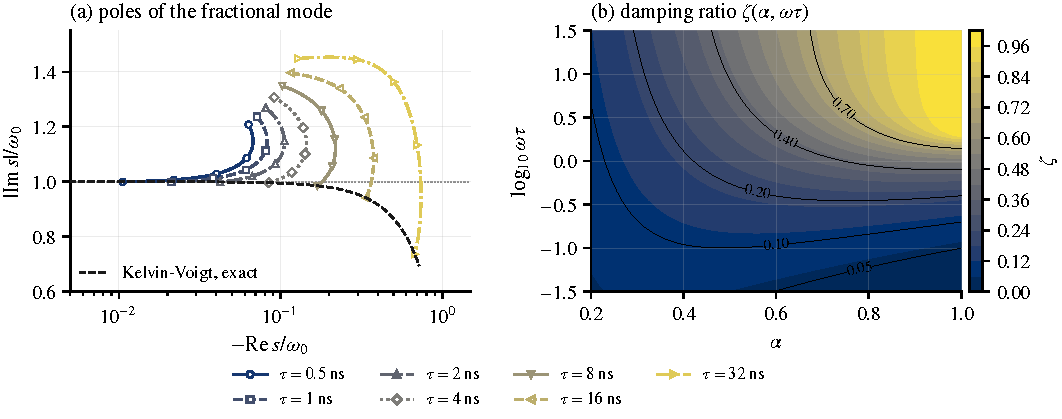
\includegraphics[width=\textwidth]{F6_damping.pdf}
\caption{Variations of (a) the pole of a mode at $f_0=\SI{6.73}{MHz}$ ($\omega_0=2\pi f_0$) over $\omega\tau=0.02$--$1.35$ for seven relaxation times, identified by $\tau$ in the legend and distinguished by line style and marker, with markers at five Caputo orders, and of (b) the damping ratio over $\omega\tau=10^{-1.5}$--$10^{1.5}$ and $\alpha=0.2$--$1$ with labeled contours, for the fractional Kelvin--Voigt element with branch continuation. The dashed arc is the exact Kelvin--Voigt locus, on which every $\alpha=1$ pole lies. Fractional poles fan upward, integer-order poles over-damp.}
\label{fig:damping}
\end{figure}

\FloatBarrier
\subsection{Window size and shape against the second moment}
\label{sec:windowshape}

Figure~\ref{fig:window} shows what the size and the shape of the window do on
a problem whose classical answer is known, which is the second design question
because the strain-gradient energy is linear in $M$: if that linearity holds,
the shape cannot matter once $M$ is fixed, and any size dependence must enter
through $M$ alone. Panel~(a) is the numerical statement of
Sec.~\ref{sec:window} on an isotropic plane-strain test problem (rectangle
$1\times0.2$, $20\times4$ mesh, uniaxial edge traction, displacement averaged
over the loaded edge), plotted against the normalized window size for an
ellipsoidal window of semi-axis $l$, a cuboidal window of half-width $l$, and a
cuboidal window scaled to carry the same $M$ as the ellipsoid,
$a=l\sqrt{3/5}$. The third curve is indistinguishable from the first: within
the adopted second-moment model the shape of the window is irrelevant at fixed
$M$. The second curve shows the error made by ignoring the distinction: equal
half-widths instead of equal $M$ over-stiffen the response, and the
discrepancy grows with the window size. Writing $L_x$ for the rectangle length, at $l/L_x=0.2$ a cuboid of half-width
$l$ retains $0.922$ of the classical loaded-edge displacement, an ellipsoid of
semi-axis $l$ retains $0.941$, and the equal-$M$ cuboid sits on the ellipsoid
curve to the third decimal. At fixed $M$ the shape of the window is therefore
immaterial to $10^{-3}$, which is the coefficient ratio $5/3$ in the gradient
stiffness seen from the response side. The assumed operating range is
$a/L\le0.2$, the right-hand edge of the figure.

Panels (b) and (c) are the corresponding static statement. The clamped strip of
Table~\ref{tab:params} is solved under an end load for three window sizes and
each solution is compared with the classical one of the same geometry and load.
The gradient terms stiffen the member. The difference against the classical
solution vanishes at the clamped edge, where both fields satisfy the same
kinematic conditions, and then accumulates along the member instead of decaying
over a thin layer: at these window sizes the gradient effect is distributed
rather than local, and its size grows with the window. That is why $a/L\le0.2$
is quoted as an assumed operating range and not as a validated truncation
threshold. Hence, at a fixed second moment the shape of the window is immaterial
to the third decimal, and its size and its anisotropy are the only window
parameters left in the model. The entries of \ref{app:Mcoeff} used here are the
ellipsoidal second moment \eqref{eq:Mellip} and its rotation \eqref{eq:Mrot}, and
the classical profile follows from \eqref{eq:limitM} with flexoelectricity
suppressed.

\begin{figure}[!htbp]
\centering
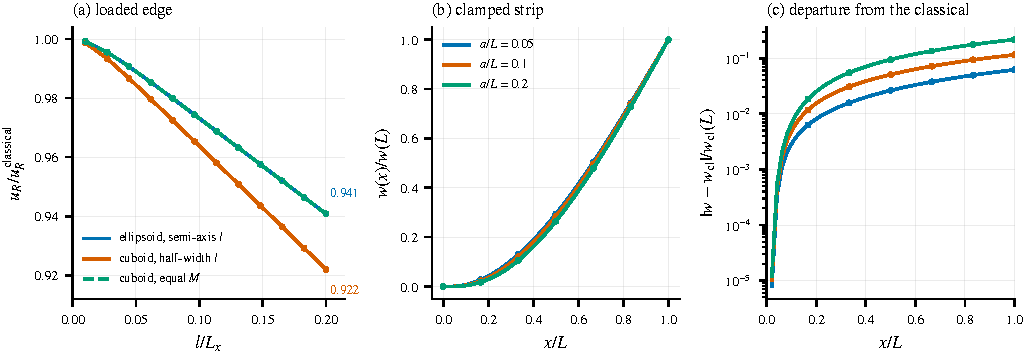
\includegraphics[width=\textwidth]{F7_window.pdf}
\caption{Variations of (a) the loaded-edge displacement of an isotropic plane-strain rectangle against normalized window size, for an ellipsoid, a cuboid of equal half-width and a cuboid of equal second moment, and of (b) the deflected shape of a clamped strip for three window sizes together with (c) its difference from the classical profile. Windows of equal second moment collapse onto one curve. Panel (a) uses a $1\times0.2$ rectangle and a $20\times4$ mesh under uniaxial edge traction; panels (b,c) use Table~\ref{tab:params} with $a/L=0.05$, $0.1$ and $0.2$.}
\label{fig:window}
\end{figure}

\FloatBarrier
\subsection{Thickness: a flexoelectric size effect against a thickness-independent
piezoelectric coupling}
\label{sec:thickness}

Figure~\ref{fig:thickness} shows whether thinning a device helps, which is the
third design question because the two available couplings scale differently
with thickness: physically, a bending mode of thickness $h$ carries a strain
gradient of order $\kappa_c/h$, so a coupling proportional to the gradient
grows as $h^{-2}$, while a coupling proportional to the strain does not grow
at all. The figure answers the question by solving the same strip at eight
thicknesses between \SI{10}{\micro\meter} and \SI{1}{\micro\meter} with a
\SI{200}{\micro\meter} length and the window held at half-widths
$3\times1$\,\si{\micro\meter}, so that the thickness is the only variable;
Table~\ref{tab:thickness} lists the sweep, and \ref{app:verification} carries
the mesh witnesses. One qualification belongs to the two thinnest points: the
window half-thickness is \SI{1}{\micro\meter} throughout, so at
$h=\SI{2}{\micro\meter}$ it is half the strip and at $h=\SI{1}{\micro\meter}$
it equals the strip. The second-moment tensor of the full window is used at
every thickness and no truncated-window boundary correction is applied, so $M$
acts there as a local effective gradient tensor rather than as the moment of a
window small compared with the body. The two panels are two electrical
configurations of that strip: panel~(a) is poled through the thickness
(electrodes on the long faces, gap $h$, $\kappa_{yy}=\kappa_{33}$) and
panel~(b) along the length (electrodes on the short faces, gap $L$,
$\kappa_{xx}=\kappa_{33}$).

\begin{figure}[!htbp]
\centering
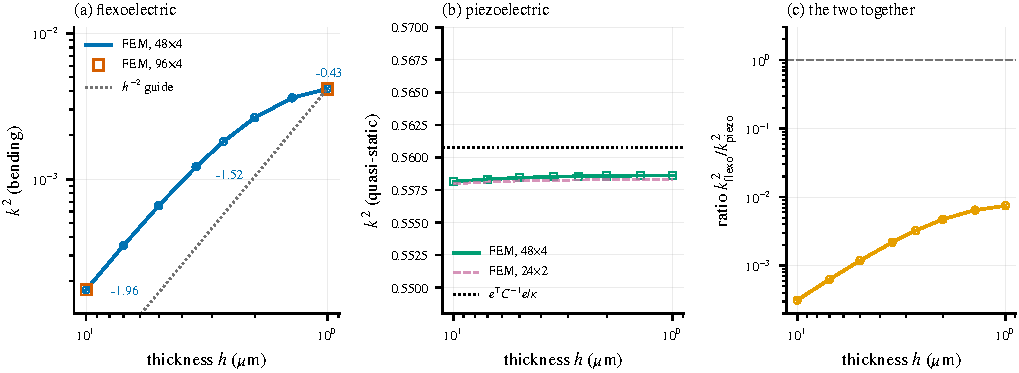
\includegraphics[width=\textwidth]{F8_thickness.pdf}
\caption{Variations of (a) the flexoelectric bending coupling against strip thickness at eight thicknesses, with local log--log slopes, a $96\times4$ witness at both ends and the $h^{-2}$ guide, of (b) the piezoelectric extensional coupling of the same strip with $\mu=0$, constant to $0.09\,\%$ over $10\to1\,\si{\micro\meter}$, and of (c) their ratio, which spans $3.1\times10^{-4}$ to $7.5\times10^{-3}$.}
\label{fig:thickness}
\end{figure}

\subsubsection{The flexoelectric size effect}

The flexoelectric coupling rises by a factor $24$ from $1.74\times10^{-4}$ at
\SI{10}{\micro\meter} to $4.2\times10^{-3}$ at \SI{1}{\micro\meter}. Its local
log--log slope is $-1.96$ at the thick end, close to the $h^{-2}$ scaling of a
gradient effect with a window much smaller than the thickness, and falls to
$-1.52$, $-1.26$ and $-0.43$ on the successively thinner pairs, the seven
segments spanning $-1.96$ to $-0.43$. The saturation survives refinement: a
$96\times4$ witness reproduces the $48\times4$ values to $0.04\,\%$ and
$0.35\,\%$ at the two ends of the range, and the residual at $\mu=0$ is
$1.0\times10^{-10}$, seven orders of magnitude below the signal. The
dimensionless group that explains the saturation is $a_2/h$, the window
half-thickness over the strip thickness, which runs from $0.10$ at
$h=\SI{10}{\micro\meter}$ to $1.0$ at \SI{1}{\micro\meter}: the slope decreases
monotonically as $a_2/h$ grows, which is what a fixed-size window does when it
smears a through-thickness gradient that becomes comparable to the strip. The
same stiffening appears in the fundamental frequency, which follows
$210.4,108.0,50.2,34.7$\,kHz where pure Euler--Bernoulli scaling from the
thickest strip would give $210,105,42,21$\,kHz.

Figure~\ref{fig:modetrack} records the mode identification behind the sweep,
which is what makes the factor $24$ a statement about one mode. The mode shape
at each thickness is compared with the one at $h=\SI{10}{\micro\meter}$ through
the modal assurance criterion, which stays above $0.999$ across the whole
sweep, and the ratio $f_2/f_1$ stays between $6.21$ and $6.27$: the branch that
carries the coupling is separated from its neighbors by the same margin at
every thickness.

\begin{figure}[!htbp]
\centering
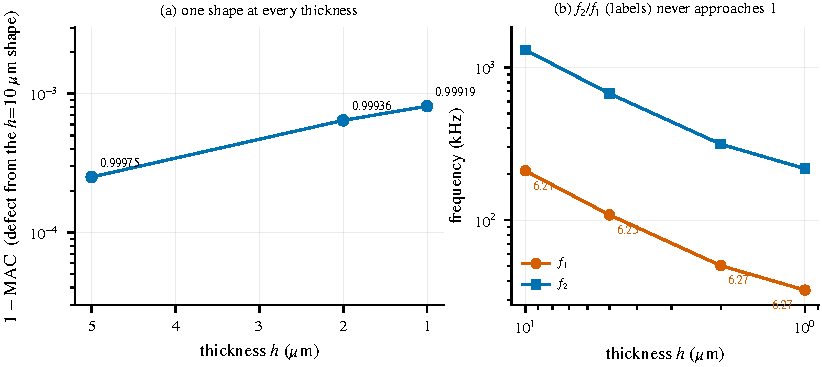
\includegraphics[width=0.90\textwidth]{FB1_tracking.pdf}
\caption{Variations of (a) the defect $1-\mathrm{MAC}$, the MAC being the modal assurance criterion, between the mode shape at each thickness and the shape at $h=\SI{10}{\micro\meter}$, with the MAC printed, and of (b) the frequencies of the first two modes and their ratio, over a sweep from $10$ to $1\,\si{\micro\meter}$. The tracked branch stays within $10^{-3}$ of itself, so the identification is unambiguous. Inputs match Fig.~\ref{fig:thickness}(a).}
\label{fig:modetrack}
\end{figure}

Figure~\ref{fig:modes} complements this one-mode identification with the
spatial structure of the tracked branch. The surface is the computed
open-circuit bending displacement, colored by the solved electric potential,
and the inset gives a labeled two-dimensional reading of the same potential on
the strip coordinates so that the through-thickness variation is not inferred
from the three-dimensional projection alone.

\begin{figure}[!htbp]
\centering
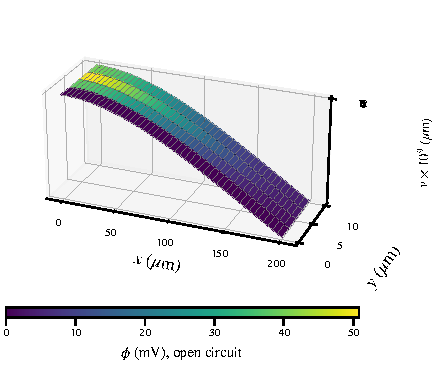
\includegraphics[width=\textwidth]{FB2_modes.pdf}
\caption{Open-circuit bending mode and its potential field. The three-dimensional surface is the computed transverse displacement in nanometers, colored by the solved electric potential; the inset shows labeled potential contours on the strip coordinates, with contour labels in millivolts. Both views use the same finite-element solution and the same assumed inputs as Fig.~\ref{fig:fields}.}
\label{fig:modes}
\end{figure}

%% generated table -- do not edit (see AUTHOR_TODO.md)
\begin{table}[!htbp]
\centering
\small
\caption{Thickness sweep behind Fig.~\ref{fig:thickness}. First frequency,
flexoelectric bending coupling and extensional coupling of the poled strip. The
bending column carries $\mu=10^{-6}$\,\si{\coulomb\per\metre}, the extensional
column $\mu=0$, and both are converged to the tolerance of
\ref{app:verification}.}
\label{tab:thickness}
\begin{tabular}{@{}r r r r@{}}
\toprule
$h$ (\si{\micro\metre}) & $f_1$ (kHz) & $k^2_{\rm flexo}$ & $k^2_{\rm piezo}$ \\
\midrule
10 & 210.4 & 1.744e-04 & 0.55814 \\
7 & 148.7 & 3.510e-04 & 0.55831 \\
5 & 108.0 & 6.587e-04 & 0.55843 \\
3.5 & 78.2 & 1.218e-03 & 0.55851 \\
2.7 & 62.9 & 1.808e-03 & 0.55855 \\
2 & 50.2 & 2.642e-03 & 0.55858 \\
1.4 & 40.3 & 3.608e-03 & 0.55860 \\
1 & 34.7 & 4.174e-03 & 0.55861 \\
\bottomrule
\end{tabular}
\end{table}


\subsubsection{The piezoelectric coupling is thickness independent}

Panel~(b) of Fig.~\ref{fig:thickness} is the counterpart of panel~(a). The
quasi-static extensional coupling takes the values $0.55814$, $0.55843$,
$0.55858$ and $0.55861$ at $10$, $5$, $2$ and \SI{1}{\micro\meter}, that is it
changes by $0.09\,\%$ between \SI{10}{\micro\meter} and \SI{1}{\micro\meter},
against the constitutive closed form $0.5608$ for the same material and the
same plane-stress kinematics. The piezoelectric effect is a bulk effect, so a
thinner strip is electromechanically neither better nor worse, whereas the
flexoelectric effect is a gradient effect and improves by a factor $24$ over
the same range. A device can therefore be thinned for the flexoelectric
response without a penalty in the piezoelectric one, and the crossover
thickness is a property of the window and of $\mu$, not of the piezoelectric
constants.

\subsubsection{What the piezoelectric terms do on the bending device}

The bending configuration is poled along $y$ with electrodes on the long faces,
and the crystal carries $e_{31}$ and $e_{33}$ as well, so the two effects can
be separated inside one run. With $\mu=0$ the piezoelectric coupling of that
mode is $1.0\times10^{-10}$ at every thickness, because the piezoelectric charge
$e_{31}\varepsilon_{xx}+e_{33}\varepsilon_{yy}$ is odd in $y-h/2$ and its
integral over a face electrode vanishes, so the arrangement carries no net
piezoelectric charge. With $e=0$ the flexoelectric coupling runs from
$1.76\times10^{-4}$ to $5.5\times10^{-3}$, a factor $31$, while the full crystal
gives the $24$ reported above: the piezoelectric terms shift the flexoelectric
coupling by up to $24\,\%$ at the thinnest strip, through the elastic stiffness
of the same mode rather than through a charge they contribute. The number
quoted in the abstract and in Fig.~\ref{fig:thickness} is the full-crystal one.

\subsubsection{Numerical reproducibility of the thinnest point}

The $h=\SI{1}{\micro\meter}$ point is the least reproducible number in the
paper. Its $k^2$ is a difference of two nearly equal eigenvalues of a pencil
whose condition number is $\sim10^{12}$ at that thickness, so the number
carries the accuracy of the eigensolver: four mathematically equivalent
eigensolver paths and four numeric stacks agree on $4.2\times10^{-3}$ and on
the factor $24$ to within $0.5\,\%$. The spread quoted is the range over the
midpoint of those equivalent results, and at $h=\SI{10}{\micro\meter}$ it is
at most $10^{-4}\,\%$. Values are quoted to two significant digits. Hence
thinning the strip multiplies the flexoelectric bending coupling by $24$ while
leaving the piezoelectric extensional coupling unchanged to $0.09\,\%$, which
is the size effect that this model was built to separate from the material
property. The estimate \eqref{eq:xflexo} is the $h^{-2}$ guide drawn in
panel~(a), and the inverse route \eqref{eq:muV} of Sec.~\ref{sec:calib_a_mu}
is the one that would measure $\mu$ rather than assume it.

\FloatBarrier
\subsection{The design map}
\label{sec:designmap}

Figure~\ref{fig:designmap} shows the two couplings of the third question on one
grid, which a designer needs because they are not comparable in size and a device
has to be designed against both at once. They depend on different variables: the flexoelectric bending coupling on the thickness and on the
window, the piezoelectric extensional coupling on neither. Figure~\ref{fig:designmap}
resolves them over the same two parameters. Panel~(a) is the flexoelectric
bending coupling on a grid of eight thicknesses and eight window
half-thicknesses, computed with the mode-based measure \eqref{eq:k2mode} and
the same $48\times4$ mesh as Fig.~\ref{fig:thickness}(a); panel~(b) is the
ratio of that bending coupling to the mode-free extensional coupling
\eqref{eq:kstatic} of the same strip. Both panels carry the line $a_2=h$, along which
the window is as thick as the strip, and the map stops at $a_2/L=0.2$, the
operating range assumed in Sec.~\ref{sec:limit_window}.

The map has three features worth naming. First, the coupling is controlled by
the ratio $a_2/h$ rather than by the thickness alone. At
$h=\SI{10}{\micro\meter}$ shrinking the window half-thickness from $1$ to
$0.25\,\mu$m changes the coupling from $1.7\times10^{-4}$ to
$1.6\times10^{-4}$, a change of $5.5\,\%$, because the window is far thinner
than the strip in both cases; at $h=\SI{1}{\micro\meter}$ the same change of
window takes the coupling from $4.2\times10^{-3}$ to $1.0\times10^{-2}$, a
factor $2.5$. Second, the window is the stronger lever of the two once it is
comparable to the strip: over the whole map the coupling spans
$3.6\times10^{-6}$ to $1.0\times10^{-2}$, of which the thickness alone
accounts for the factor $24$ of Fig.~\ref{fig:thickness}(a). Third, the two
couplings never become comparable at these parameters: the ratio in panel~(b)
spans $6.5\times10^{-6}$ to $1.9\times10^{-2}$, and it reaches $0.1\,\%$ only
below $h=5.5\,\mu$m for the window of the paper, $a_2=\SI{1}{\micro\meter}$.
The map is quoted to two significant digits because its thin-strip entries are
differences of nearly equal eigenvalues and move in the third digit across
numeric stacks.
The design rule that follows is that the window should be chosen for the
gradient one wants to resolve and the thickness for the size effect one wants
to exploit; and that a device in which the two couplings are meant to compete
needs a window thinner than the strip and a flexoelectric coefficient two
orders of magnitude larger than the value assumed here. The map therefore distinguishes the effect of thickness from the suppression
caused by the gradient stiffness.

\begin{figure}[!htbp]
\centering
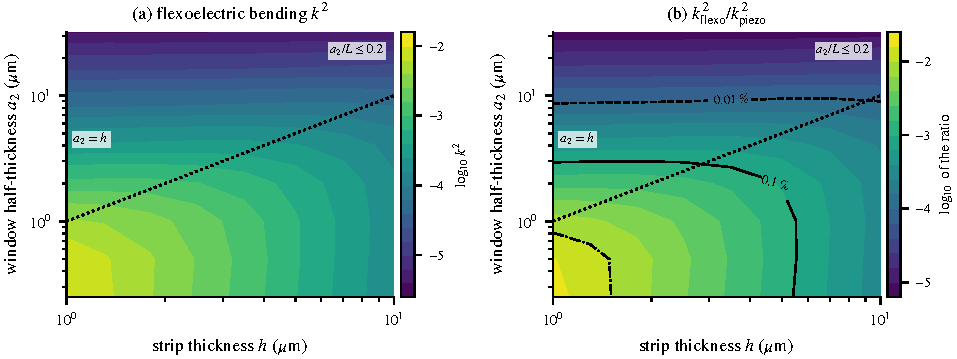
\includegraphics[width=\textwidth]{F11_designmap.pdf}
\caption{Variations of (a) the flexoelectric bending coupling and of (b) its ratio to the piezoelectric extensional coupling over strip thickness and window half-thickness, for $L=\SI{200}{\micro\meter}$ and $a_1=\SI{3}{\micro\meter}$, with the $0.01\,\%$ and $0.1\,\%$ contours. The dotted line is $a_2=h$ and the map ends at the assumed $a_2/L=0.2$.}
\label{fig:designmap}
\end{figure}

\FloatBarrier
\subsection{Transient response and the memory model}
\label{sec:transient}

Figure~\ref{fig:ringdown} shows the ring-down of the extensional mode in the
time domain, which is the memory question of Sec.~\ref{sec:memorystudy} seen as
a device records it, because a damping ratio is a frequency-domain summary and a
sensor is read in time. The strip starts from a tip displacement of
\SI{10}{\nano\meter} and is followed for eight Caputo orders between
$\alpha=1$ and $0.4$ at fixed $\tau=\SI{3}{\nano\second}$
($\omega\tau=0.13$): the tip displacement in panel~(a) and the open-circuit
voltage in panel~(b). The initial voltage, \SI{139}{\volt}, is set by the mode
shape and the electrode configuration and is independent of $\alpha$, as it
must be, since the memory term vanishes at $t=0^{+}$; the decay rate, by
contrast, depends on $\alpha$. The $\alpha=1$ curve is the exponential decay of
the classical Kelvin--Voigt element, while the fractional curves are not
exponential, and it is that difference which the damping map of
Fig.~\ref{fig:damping}(b) quantifies. Over the eight orders plotted, the
decrement of the tip displacement over the first two peaks, converted with
\eqref{eq:zeta}, runs from $0.063$ at $\alpha=1$ to a maximum of $0.104$ at
$\alpha=0.6$ and back to $0.085$ at $\alpha=0.4$
(Table~\ref{tab:ringdown}). For $\alpha<1$ it is a first-period decrement and
not a damping ratio, because those records are not exponential; a design that
takes the integer-order early decay as representative is in error by $64\,\%$
at $\alpha=0.6$, and the sign of the error cannot be guessed from $\alpha$
alone. Hence a recorded ring-down identifies the pair $(\alpha,\tau)$ only if
the order is known from an independent measurement, which is the route taken in
Sec.~\ref{sec:calibration}. The march is the one of \eqref{eq:newmark} with the
L1 history, and the decrement is converted with \eqref{eq:zeta}.

\begin{figure}[!htbp]
\centering
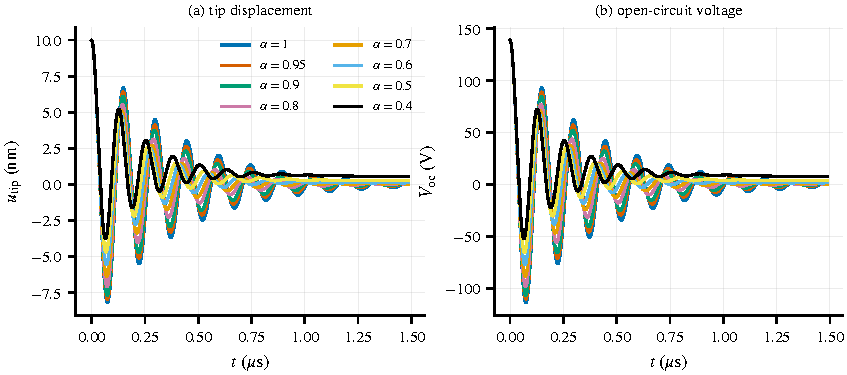
\includegraphics[width=\textwidth]{F9_ringdown.pdf}
\caption{Variations of (a) the tip displacement and (b) the open-circuit voltage of the extensional mode at \SI{6.727}{MHz} for eight Caputo orders, with modal memory on $K_{\rm eff}$, eight modes, $\tau=\SI{3}{\nano\second}$ ($\omega\tau=0.13$), an initial tip displacement of \SI{10}{\nano\meter} and $4000$ L1 steps over ten periods. Only the $\alpha=1$ decay is exponential.}
\label{fig:ringdown}
\end{figure}

\FloatBarrier
\subsection{Application: a \SI{200}{\micro\meter} by \SI{10}{\micro\meter}
strip in open-circuit sensing}
\label{sec:application}

The worked case is a \SI{200}{\micro\meter} long, \SI{10}{\micro\meter} thick
$\mathrm{BaTiO_3}$ strip clamped on one short edge, poled along its length and
electroded on the two ends: the strain in the active region is extensional, so
the piezoelectric coupling dominates and the flexoelectric term is a
size-dependent correction. Table~\ref{tab:application} collects the four
polarization/kinematics combinations of that strip, each solved from the
condensed system \eqref{eq:saddle} with the electrode charge
\eqref{eq:electrode}, and each quoted using the mode-based coupling \eqref{eq:k2mode}. The lowest-frequency mode of the
extensional configuration is at \SI{147.73}{kHz}, above the clamped-free value
of a beam of the same length because the gradient terms stiffen the member,
while the strongly coupled extensional mode sits at \SI{6725.8}{kHz}.

\begin{table}[!htbp]
\centering
\small
\caption{The coupling of the strongest mode, its frequency and the
open-circuit voltage at \SI{10}{\nano\meter} of tip motion, for a
\SI{200}{\micro\meter}$\times$\SI{10}{\micro\meter} strip in four polarization
and kinematics combinations. The two plane-stress rows are the configurations
of Fig.~\ref{fig:geometry}, and the couplings of the four rows are not
additive.}
\label{tab:application}
% table generated from the archived results
\begin{tabular}{@{}llcccc@{}}
\toprule
poling & kinematics & mode & $f$ (kHz) & $k^2$ & $V$ at \SI{10}{\nano\metre} (V) \\
\midrule
y & plane strain & bending (4) & 6721.8 & 0.1749 & 3.48 \\
y & plane stress & bending (4) & 6361.0 & 0.1141 & 2.41 \\
x & plane strain & extensional (5) & 7161.0 & 0.4024 & 141.45 \\
x & plane stress & extensional (5) & 6725.8 & 0.4580 & 138.99 \\
\bottomrule
\end{tabular}

\end{table}

Three consequences follow.

\begin{enumerate}
\item \textbf{The electrode arrangement dominates.} Poling along the length
  gives $k^2=0.4580$ and \SI{138.99}{\volt} at \SI{10}{\nano\meter} of motion;
  the bending configuration gives $0.1141$ and \SI{2.41}{\volt} -- a factor
  $58$ in voltage at equal amplitude and a factor four in $k^2$. The handicap
  belongs to the arrangement, not to $e_{31}$: a symmetric strip bent between
  full through-thickness electrodes collects almost no net charge.
\item \textbf{The quasi-static coupling is $0.5581$} and thickness independent
  (Sec.~\ref{sec:thickness}): the number to quote far below the first
  resonance, and the one that survives thinning.
\item \textbf{The damping is set by $(\alpha,\tau)$ and by the memory matrix},
  not by a material constant: at $\omega\tau=0.3$ and $\alpha=1$,
  $\zeta_{\rm eff}=0.15003$ on $K_{\rm eff}$ against $0.0675$ on $K_{uu}$, a
  ratio of $0.450$. A damping number quoted without $\alpha$, $\tau$ and the
  memory matrix is under-specified.
\end{enumerate}

These numbers are the output of the model, and each of them rests on an input
that no constitutive table supplies; Sec.~\ref{sec:calibration} identifies those
inputs one at a time and states the ranges over which the numbers hold.

\FloatBarrier

%% ===========================================================================
\FloatBarrier
\section{Parameter identification and limitations}
\label{sec:calibration}
%% ===========================================================================

Four parameters are supplied by no constitutive table: the window size $a$,
the fractional order $\alpha$, the relaxation time $\tau$ and the flexoelectric
coefficient $\mu$. This section states how each is obtained from a separate
observable and over which ranges the results of Sec.~\ref{sec:results} hold, so
that a reader can tell a measured input from an assumed one.

\FloatBarrier
\subsection{Measurement routes for the four parameters}
\label{sec:calib_a_mu}

The four are not of the same kind. The geometry of the interaction, $M_{mn}$
and the orientation $\theta$ of its principal axes, comes from size-effect and
texture measurements; the material response, $\alpha$ and $\tau$, from
dielectric loss; $\mu$ from a bending or a direct charge measurement. The
protocol is ordered so that each step fixes one quantity and the later steps
verify the parameters fixed in preceding steps, as in the
characteristic-length identification of the one-scale theory~\cite{fem1}.

\begin{enumerate}
\item Bending of strips cut along $x$ and $y$ at three or more thicknesses in
  $h/\sqrt{M_{22}}\in[2,20]$: the ratio of apparent to classical compliance
  against $h$ fixes $M_{22}$ through the thickness.
\item The same strips cut at $0^\circ,15^\circ,\dots,90^\circ$: the compliance
  and the first frequency against the cut angle fix $M_{11}/M_{22}$ and the
  orientation $\theta$.
\item Ultrasonic dispersion: the phase velocity $c(k)$ over the band in which
  the gradient term is visible fixes $\tfrac14 M_{mn}$ without any boundary
  condition.
\item A boundary-layer profile by digital image correlation: the decay length
  of the strain at a clamped edge fixes $M_{22}$ from one specimen.
\item An image of the microstructure: integrating $s_ms_n$ over the
  reconstructed window fixes the anisotropy of $M$ directly.
\item Specimens spanning the aspect ratio and the window angle: the coupling
  factor and the first frequency against both are then a prediction, not a fit.
\item The reconstructed two-point correlation: its decay lengths set the
  adequacy of the second-moment description, which this paper assumes and does
  not test.
\end{enumerate}

Steps 1, 3 and 4 determine $M_{22}$ from three independent observables, so
agreement among them checks the second-moment description instead of repeating
one measurement; step~6 turns the calibrated tensor into a prediction of
Figs.~\ref{fig:orientation} and~\ref{fig:design}; step~7 is the test of the
description itself and is the open problem of the model.

\paragraph{The flexoelectric coefficient} The direct route is a four-point
bending test on a poled bar with electrodes on the two faces: for the geometry
of Fig.~\ref{fig:geometry}(a) the open-circuit voltage at a known curvature
$\kappa_{c}$ is
\begin{equation}
  V = \frac{\mu\,\kappa_{c}\,h}{\kappa_{33}},
  \label{eq:muV}
\end{equation}
with no discretization involved and $\kappa_{33}=4.9583\times10^{-10}$\,\si{
\farad\per\meter} the polar-axis permittivity of \eqref{eq:D}. The inverse route
measures the charge released by a device whose curvature is known from its
deflection. Both fix the magnitude, which is linear in $\mu$; the sign comes
from the crystal symmetry. The value used here,
$\mu=10^{-6}$\,\si{\coulomb\per\meter}, is the order reported for perovskite
ceramics, and Sec.~\ref{sec:material} states once how every flexoelectric
coupling below follows it.

\FloatBarrier
\subsection{Identification of the fractional order and of the relaxation time}
\label{sec:calib_alpha_tau}

The pair $(\alpha,\tau)$ comes from a dielectric loss measurement. The
fractional Kelvin--Voigt element \eqref{eq:kvfreq} has
\begin{equation}
  \tan\delta=\frac{(\omega\tau)^{\alpha}\sin(\pi\alpha/2)}
     {1+(\omega\tau)^{\alpha}\cos(\pi\alpha/2)},
  \label{eq:tandelta}
\end{equation}
which increases monotonically to $\tan(\pi\alpha/2)$ and has no maximum, and
both $|K^{*}|/K$ and $\tan\delta$ are monotone in $\omega\tau$; so no single
frequency carries $\tau$, and the pair $(|K^{*}|/K,\tan\delta)$ over two
decades is fitted with $(\alpha,\tau)$. At $\omega\tau=1$ the loss is
$\tan(\pi\alpha/4)$, which gives $\alpha$ from one decade once $\tau$ is known.
The ring-down gives the same information in the time domain, but not from one
number: for small loss
\begin{equation}
  \zeta=\frac{(\omega\tau)^{\alpha}\sin(\pi\alpha/2)}{2}
  \quad\Longrightarrow\quad
  \delta\approx\pi(\omega\tau)^{\alpha}\sin(\pi\alpha/2),
  \label{eq:zetasmall}
\end{equation}
so at $\alpha=1$, $\delta=\pi\omega\tau$, which reproduces \eqref{eq:zeta} to
the $1.2\,\%$ of the small-loss approximation. A single decrement fixes only
that product, so the pair needs two frequencies or one decrement at a known
$\omega\tau$.

Two cautions follow from Sec.~\ref{sec:memorystudy}: the calibration must say
which matrix the memory multiplies, since one measured decrement gives two
different $(\alpha,\tau)$ pairs under $K_{\rm eff}$ and $K_{uu}$ (their damping
ratios differ by the factor $0.450$ at $\alpha=1$); and the fit is valid only
where the measurement is -- a broadened single-power-law loss. Two well
separated loss peaks need two elements.

\FloatBarrier
\subsection{Positioning}
\label{sec:positioning}

Three lines of work meet in this paper and none of them carries all of its
ingredients. The one-scale gradient theory~\cite{fem1} supplies the $C^1$
Bogner--Fox--Schmit technology and the geometric meaning of the length tensor,
for an elastic solid without electromechanical coupling. The
polarization-gradient theory of Mindlin~\cite{Mindlin1968} and the
flexoelectric implementations that followed it~\cite{ChenYaoYvonnet2023,
JoshanSantapuri2024,Wang2024PhaseField} supply the electromechanical coupling,
with a scalar or a fitted gradient length and without dielectric memory.
Fractional constitutive models~\cite{BagleyTorvik1983,Koeller1984,
EnelundLesieutre1999} supply the broad relaxation spectrum, in mechanical
settings that have no strain gradient and no electrodes. What this paper adds
is the combination and the two consequences of the combination: the window
enters as a tensor that can be measured from a microstructure, the memory
matrix becomes an explicit modeling choice with a measurable consequence
($0.450$ on the damping ratio at $\alpha=1$), and the coupling factor of a
strain-gradient electromechanical strip is separated into a material property
($0.5581$, thickness independent) and a size effect (a factor $24$).

\FloatBarrier
\subsection{Validity window}
\label{sec:limit_window}

Three inequalities bound the results, and each is a modeling assumption rather
than a numerical tolerance.

\begin{enumerate}
\item \emph{Small coupling at the operator level.} \eqref{eq:kstatic} is used
  with the uncoupled denominator only where $k^{2}\ll1$; here
  $k^{2}=0.5581$, which is \emph{not} small, so the coupled denominator is used
  and the uncoupled form appears only in the comparison with the closed form.
\item \emph{Small window.} The truncation \eqref{eq:Mdef} is written for a
  window small against the length over which the strain gradient varies, and
  for the strip of Table~\ref{tab:params} we take $a/L\le0.2$. That is an
  assumed operating range, not a validated truncation threshold: with no
  experiment and no exact averaging operator available, nothing here fixes
  where the truncation fails. What Fig.~\ref{fig:window}(a) shows is that
  inside the range the retained second moment reproduces the exact average to
  a fraction of a per cent on every mesh, which makes the model
  \emph{self-consistent} there and is all that is claimed.
\item \emph{Operating band.} The damping map is claimed for $\omega\tau\le1$,
  the band in which the spring-pot relaxes around the device frequency. Beyond
  it the map extrapolates the fitted law, and the integer-order alternative
  departs from it by the factors quoted in Sec.~\ref{sec:memorystudy}.
\end{enumerate}

\FloatBarrier
\subsection{Limitations}
\label{sec:limitations}

The formulation is two-dimensional with a plane-stress reduction, which is a
modeling choice: plane strain would change the extensional coupling to
$0.5132$, and the three-dimensional solution differs from both, so the
thin-strip results of Sec.~\ref{sec:thickness} are two-dimensional results. Of
the inputs, two are not material constants of this crystal. The density
rescales every frequency by a common factor, so the kilohertz numbers of
Secs.~\ref{sec:orientation} and~\ref{sec:application} move while the ratios
stand. The flexoelectric coefficient scales every flexoelectric coupling as
$\mu^{2}$, so the growth factor, the saturation and the comparison with the
piezoelectric response are unaffected while the absolute coupling is not.

The precision of Sec.~\ref{sec:thickness} is a limitation as much as a result:
two significant digits of that coupling are resolved, and the same holds, less
visibly, for any difference of nearly equal eigenvalues. The verification of
Secs.~\ref{sec:verification} and~\ref{app:verification} shows that the
implementation solves the stated equations; it does not show that they
describe a particular material, which needs the measurements of
Secs.~\ref{sec:calib_a_mu} and~\ref{sec:calib_alpha_tau}.

\FloatBarrier

%% ===========================================================================
\FloatBarrier
\section{Conclusions}
\label{sec:conclusions}
%% ===========================================================================

The formulation combines piezoelectric and flexoelectric coupling with
fractional memory in a $C^1$ Bogner--Fox--Schmit discretization. The second
moment of the averaging window sets the gradient stiffness, while modal L1
integration retains the dielectric history. The principal findings are:

\begin{itemize}
\item \textbf{The averaging window, through its second-moment tensor $M$,
  supplies the internal length.} Physically, the window is the domain over which
  the microstructure is averaged, and because the gradient energy is linear in
  $M$ the shape of that domain is not a parameter: windows of equal second
  moment give identical solutions to the third decimal, while their size spans
  the coupling from $3.6\times10^{-6}$ to $1.0\times10^{-2}$ over the map
  computed here. Rotating an anisotropic window changes the extensional
  coupling by $15$--$19\,\%$ between the aligned and transverse positions,
  because the gradient stiffness samples different directional strain gradients.
\item \textbf{The thickness $h$} converts a curvature into a strain gradient
  of order $\kappa_c/h$ and thereby separates the two couplings: the
  flexoelectric bending coupling grows by a factor $24$ between
  \SI{10}{\micro\meter} and \SI{1}{\micro\meter}, while the piezoelectric
  extensional coupling stays constant to $0.09\,\%$ and its quasi-static value,
  $0.5581$, lies within $0.5\,\%$ of the closed form $0.5608$.
\item \textbf{The flexoelectric coefficient $\mu$}, the polarization produced by
  a unit strain gradient, fixes the absolute size of the bending coupling: at
  the assumed $\mu=10^{-6}$\,\si{\coulomb\per\meter} the ratio of the two
  couplings spans $3.1\times10^{-4}$ to $7.5\times10^{-3}$ and reaches
  $0.1\,\%$ only below $h=5.5\,\si{\micro\meter}$.
\item \textbf{The Caputo order $\alpha$}, which measures how broad the
  relaxation spectrum is, controls the shape of the decay: the first-period
  decrement of the tip displacement runs from $0.063$ at $\alpha=1$ to $0.104$
  at $\alpha=0.6$ and back to $0.085$ at $\alpha=0.4$, so a free decay is not
  exponential below $\alpha=1$ and an integer-order reading is in error by
  $64\,\%$ at $\alpha=0.6$.
\item \textbf{The relaxation time $\tau$}, which places the loss peak at
  $\omega\tau$ of order unity, fixes where that damping acts: at $\alpha=1$ and
  $\omega\tau=0.3$ the damping ratio is $0.15003$ on the condensed matrix
  against $0.0675$ on the short-circuit one, a ratio of $0.450$, and the
  Kelvin--Voigt limit is reproduced to $0.02\,\%$.
\item \textbf{The element that carries all of it}, a $C^1$ Bogner--Fox--Schmit
  rectangle, converges at the $N^{-2}$ rate of bicubic Hermite interpolation, so
  that $48\times4$ elements reproduce the coupling factor to
  $6.2\times10^{-4}$ relative.
\end{itemize}

For sensing design, select the electrodes first ($0.4580$ against $0.1141$
at equal tip motion), then the thickness and window geometry; interpret decay
with $\alpha$, $\tau$ and the memory matrix stated together. Applications
remain conditional on the assumed inputs and two-dimensional kinematics:
plane-stress coupling differs from the three-dimensional value by $2.8\,\%$,
motivating measured-window calibration and shell extensions.

\FloatBarrier


\section*{CRediT authorship contribution statement}
\textbf{Author one (name to be supplied):} Conceptualization, Methodology,
Software, Validation, Formal analysis, Investigation, Writing -- original
draft. \textbf{Author two (name to be supplied):} Conceptualization, Software,
Writing -- review and editing, Supervision. \textbf{Author three (name to be
supplied):} Formal analysis, Validation, Writing -- review and editing.
\textbf{Author four (name to be supplied):} Methodology, Resources, Funding
acquisition. All authors have read and approved the final manuscript.

\section*{Declaration of competing interest}
The authors declare that they have no known competing financial interests or
personal relationships that could have appeared to influence the work reported
in this paper.

\section*{Data availability}
The numerical values behind the quantitative figures are listed in the tables
of \ref{app:data}. The material constants, the geometry and the discretization
used to obtain them are stated in Table~\ref{tab:params} and
\ref{app:verification}; the scripts and archived JSON data that reproduce them
are part of the accompanying source archive.

%% TODO  sanction number to be confirmed against the sanction letter before
%% submission.
\section*{Acknowledgements}
This research was supported by the Haryana State Research Fund (HSRF) under
sanction 14/66-2026 SPD/HSHEC/HSRF-(38), dated 13 July 2026.

\appendix
\renewcommand{\thetable}{\Alph{section}.\arabic{table}}
\renewcommand{\thefigure}{\Alph{section}.\arabic{figure}}

%% ===========================================================================
\section{Coefficients of the rectangular, elliptical and ellipsoidal averaging
windows}
\label{app:Mcoeff}
%% ===========================================================================

For a uniform kernel over a window $\mathcal{W}$ centred at the origin, the
normalised second moment is
\begin{equation}
  M_{mn} = \frac{1}{|\mathcal{W}|}\int_{\mathcal W} s_m s_n \,\mathrm{d}\bm{s},
  \label{eq:appM}
\end{equation}
which is diagonal for a window whose axes are aligned with the coordinate axes
and which transforms as $M\mapsto RMR^{\mathsf T}$ under a rotation $R$ of the
window. The three closed forms used in the paper follow from
\eqref{eq:appM} by elementary integration.

\paragraph{Cuboid.} For $\mathcal W=[-a_1,a_1]\times[-a_2,a_2]$ the area is
$4a_1a_2$ and
\begin{equation}
  M_{11} = \frac{1}{4a_1a_2}\int_{-a_1}^{a_1}\!\!\int_{-a_2}^{a_2}
           s_1^{2}\,\mathrm{d}s_1\,\mathrm{d}s_2
         = \frac{1}{4a_1a_2}\cdot 2a_2\cdot\frac{2a_1^{3}}{3}
         = \frac{a_1^{2}}{3},
  \label{eq:Mcub}
\end{equation}
and identically $M_{22}=a_2^{2}/3$; the off-diagonal integral vanishes by the
oddness of $s_1s_2$. A three-dimensional cuboid of half-widths $a_i$ gives the
same coefficient along each axis.

\paragraph{Ellipse.} For $\mathcal W=\{s: (s_1/a_1)^{2}+(s_2/a_2)^{2}\le1\}$ the
area is $\pi a_1a_2$ and the polar second moment of the semi-axis is
$\int_{\mathcal W}s_1^{2}\,\mathrm{d}A = \pi a_1^{3}a_2/4$, so that
\begin{equation}
  M_{11} = \frac{\pi a_1^{3}a_2/4}{\pi a_1a_2} = \frac{a_1^{2}}{4},
  \qquad M_{22}=\frac{a_2^{2}}{4}.
  \label{eq:Mell}
\end{equation}

\paragraph{Ellipsoid.} For the three-dimensional ellipsoid of semi-axes $a_i$
the volume is $4\pi a_1a_2a_3/3$ and
$\int_{\mathcal W}s_1^{2}\,\mathrm{d}V = 4\pi a_1^{3}a_2a_3/15$, hence
\begin{equation}
  M_{11} = \frac{a_1^{2}}{5},\qquad
  M_{22}=\frac{a_2^{2}}{5},\qquad
  M_{33}=\frac{a_3^{2}}{5}.
  \label{eq:Mellip}
\end{equation}

\paragraph{Equal-second-moment windows.} Equations~\eqref{eq:Mcub}--\eqref{eq:Mellip}
are the reason the shape of the window drops out of the model. A cuboid of
half-width $a$ and an ellipsoid of semi-axis $l$ carry the same second moment
when $a^{2}/3=l^{2}/5$, that is when $a=l\sqrt{3/5}$; for an ellipse the same
condition reads $a=l\sqrt{3/4}$. Two windows related in this way produce the
same gradient stiffness $K_g$ and therefore the same solution, which is what
Fig.~\ref{fig:domain} and the polar panel of Fig.~\ref{fig:petals} show
numerically, and what the ratio $5/3$ between the coefficients of an equal
half-width pair expresses analytically.

\paragraph{Rotated window.} A rectangular window whose long axis makes an angle
$\theta$ with $x$ has
\begin{equation}
  M_{11}(\theta) = M_{11}\cos^{2}\theta + M_{22}\sin^{2}\theta,\qquad
  M_{22}(\theta) = M_{11}\sin^{2}\theta + M_{22}\cos^{2}\theta,\qquad
  M_{12}(\theta) = \tfrac12\left(M_{22}-M_{11}\right)\sin2\theta,
  \label{eq:Mrot}
\end{equation}
so that the off-diagonal coupling is largest at $\theta=45^\circ$ and vanishes
when the window is aligned with the axes. This is the tensor that the
orientation sweep of Sec.~\ref{sec:orientation} rotates.

\paragraph{Reduction to a scalar length.} The ellipsoid gives the coefficient
that the one-scale theory of the authors' earlier work carries:
$M_{mn}=L_{mn}/5$, hence $\tfrac14M_{mn}=\tfrac1{20}L_{mn}$ and the gradient
energy of~\cite{fem1} is recovered exactly, and setting
$M_{mn}=\ell^{2}\delta_{mn}$ reduces the same expression to the isotropic
Aifantis form, for which the boundary-layer length of a clamped bar is
$\sqrt{\ell^{2}/2}$, the value that follows from putting $L_{mn}=5\ell^{2}
\delta_{mn}$ in the $\sqrt{L/10}$ of the one-scale theory.

%% ===========================================================================
\FloatBarrier
\section{Benchmarks and convergence study}
\label{app:verification}
\setcounter{table}{0}
\setcounter{figure}{0}
%% ===========================================================================

This appendix collects the benchmarks behind Sec.~\ref{sec:verification} in
full: the benchmark, identity and independent-route record, and the
convergence study. The numerical precision of the thinnest point follows the
two tables.

Table~\ref{tab:verification} lists the benchmark problems, the exact
identities and the tolerance each was required to meet, together with the value
obtained. The identities are the ones that a re-implementation can reproduce
without any of the data of this paper: the patch-test energy of a constant
strain field, the second-moment coefficients of \ref{app:Mcoeff}
recovered from a numerical integration of the window, the closed-form coupling
factor of a uniaxial crystal, and the analytical damping ratio of the classical
Kelvin--Voigt element. The rows marked as independent routes are values
recomputed along a path that does not use the assembled matrices at all --
Euler--Bernoulli theory for the bar frequency, the constitutive tensors for the
coupling factor, the closed forms of \ref{app:Mcoeff} for the window
coefficients, and the analytical limit for the damping ratio.

\begin{table}[!htbp]
\centering
\small
\caption{Verification record: benchmarks, exact identities and independent
routes, each with the value obtained and the tolerance it was required to
meet. The material, the geometry and the mesh of each row are those of
Sec.~\ref{sec:material}.}
\label{tab:verification}
%% A compact list of the numerical benchmarks: what was computed, what it is
%% compared with, and the agreement.
\begin{tabular}{@{}l l l@{}}
\toprule
check & obtained & reference \\
\midrule
patch test, relative energy error & $4.44\times10^{-16}$ & $0$ \\
gradient energy at constant strain & $1.06\times10^{-12}$ & $0$ \\
$K_g$ of the ellipsoid vs closed form & $3.40\times10^{-16}$ & $0$ \\
$K_g$(cuboid)$/K_g$(ellipsoid), equal half-width & 1.666667 & $5/3$ \\
equal-$M$ cuboid and ellipsoid, max rel.\ difference & $0$ & $0$ \\
tip displacement, length-scale sweep & 4.2339\,\si{\micro\meter} & 4.23\,\si{\micro\meter} \\
observed order of convergence & 1.68 & $2.01$ on the finest pair \\
piezoelectric $k^2$ of extensional mode 5, plane strain vs plane
stress & 0.4024 vs 0.4580 & mode 5 of each model, MAC $0.99999$ \\
L1 order at $\alpha=1$ & 0.99 & $1$ \\
free strip $k^2$, FEM vs 2-D closed form & 0.56079 vs 0.56079 & $<10^{-3}$ rel. \\
free strip, 3-D vs 2-D reduction & 2.83\,\% & modeling gap \\
clamped strip, $96\times4$ vs $48\times4$ & 0.55992 vs 0.55957 & $6.2\times10^{-4}$ rel. \\
flexoelectric energy, uniform curvature & $3.570415\times10^{-4}$ & $3.570415\times10^{-4}$ \\
open-circuit voltage, uniform curvature & $1.7\times10^{-13}$\,\si{\volt} & $<10^{-10}$\,\si{\volt} \\
clamped-free $f_1$, FEM vs Euler--Bernoulli & 144.6 vs 143.8\,\si{\kilo\hertz} & $128\times4$: 144.08 \\
clamped-clamped $f_1$, FEM vs Euler--Bernoulli & 919.2 vs 915.0\,\si{\kilo\hertz} & $48\times4$ \\
modal truncation, 24 modes & $3.19\times10^{-2}$ & monotone in $N$ \\
\bottomrule
\end{tabular}

\end{table}

The two closed forms of Sec.~\ref{sec:verification} rest on the scalar
$e^{\mathsf T}C^{-1}e=6.3308\times10^{-10}$ of the reduced tensors, and the
\SI{0.5}{\percent} agreement between them and the finite element value is the
agreement of that scalar with the assembled route rather than a coincidence of
two discretizations.

The clamped--free frequency is the one row with an exact counterpart, so it is
also reported under refinement: the $128\times4$ mesh gives
144.08\,\si{\kilo\hertz}, against 144.6\,\si{\kilo\hertz} on the
$48\times4$ mesh and 143.8\,\si{\kilo\hertz} from Euler--Bernoulli theory.

The two-dimensional reduction is quantified in the same record: the
plane-stress coupling differs from the three-dimensional value by $2.8\,\%$,
which is the size of the modeling error that the reduction introduces and the
reason the two reductions are not used interchangeably. Of the independent
values, the damping ratio of the element at $\alpha=0.3$ and $\omega\tau=0.3$
is $0.108$, against a peak of $0.179$ at $\alpha=0.7$
(Sec.~\ref{sec:memorystudy}).

Two rows of Table~\ref{tab:verification} are comparisons rather than exact
identities. The order of convergence is the least-squares slope of
$\log|u_R/u_{\rm ref}-1|$ against $\log h$, with $h=L/n_x$ halved over the
four meshes $5\times1$, $10\times2$, $20\times4$ and $40\times8$ of the
gradient-free benchmark of Sec.~\ref{sec:verification}; the slope over all
four is 1.68 and the finest pair alone gives 2.01, so the sequence is entering
its asymptotic range from the coarse end. The expected rate for the bicubic
Hermite rectangle is $O(h^{4})$ in $L^2$ and $O(h^{3})$ in $H^1$ on a smooth
solution, and a linear functional such as $u_R$ converges at least as fast as
the energy norm; the requirement is the empirical slope above 1.5, and no
theoretical exponent is claimed beyond that bound. The extensional coupling is
compared across the two reductions on the same $24\times2$ mesh: $0.4024$ in
plane strain against $0.4580$ in plane stress. The two models are compared
mode by mode before the couplings are, because the two reductions could in
principle select different shapes and then the comparison would be empty. They
do not: the shape selected by the rule of Table~\ref{tab:application} is mode
5 in both, and the two short-circuit mode shapes, mass-normalized, overlap
with $\mathrm{MAC}=0.99999$, while the largest overlap between different
members of the two six-mode sets is $2.8\times10^{-6}$. The coupling therefore
differs by the elastic reduction alone, which stiffens the section and lowers
$k^{2}=e^{2}/(C\kappa)$; the difference is a property of the model.

Table~\ref{tab:convergence} is the convergence study behind
Fig.~\ref{fig:convergence}. The frequency of the extensional mode and its
mode-free coupling factor are listed for four meshes, with the errors referred
to the $48\times4$ mesh used in the paper: the coarser $24\times2$ mesh of the
parameter sweeps differs from it by $0.04\,\%$ in frequency and by
$0.03\,\%$ in the coupling factor, and the other two rows by less. None of
the four rows is a clamped strip; the
clamped strip is the $96\times4$ against $48\times4$ entry of
Table~\ref{tab:verification}, whose coupling factors differ by
$6.2\times10^{-4}$ relative.

%% generated table -- do not edit (see AUTHOR_TODO.md)
\begin{table}[!htbp]
\centering
\caption{Convergence of the extensional mode behind
Fig.~\ref{fig:convergence}: strip \SI{200}{\micro\meter}$\times$\SI{10}{\micro\meter},
poling $x$, plane stress, $\mu=0$, $a_1\times a_2=3\times1$\,\si{\micro\meter}.
The frequency is that of the extensional mode of the short-circuit eigenvalue
problem and the coupling is the mode-free quasi-static value of
\eqref{eq:kstatic}, the number quoted in the text; the errors are referred to
the $48\times4$ mesh.}
\label{tab:convergence}
\begin{tabular}{@{}l r r r r r@{}}
\toprule
mesh & dof & $f$ (kHz) & $k^2$ & err $f$ & err $k^2$ \\
\midrule
$12\times2$ & 312 & 4745.4 & 0.55682 & 3.2e-03 & 2.4e-03 \\
$24\times2$ & 600 & 4732.0 & 0.55797 & 3.7e-04 & 3.0e-04 \\
$36\times2$ & 888 & 4730.0 & 0.55814 & 3.7e-05 & 7.0e-06 \\
$48\times4$ & 1960 & 4730.2 & 0.55814 & 0.0e+00 & 0.0e+00 \\
\bottomrule
\end{tabular}
\end{table}


\paragraph{Numerical precision of the thinnest point} The
$h=\SI{1}{\micro\meter}$ coupling is a difference of two nearly equal
eigenvalues of a pencil whose condition number is $\sim10^{12}$, so it
inherits the accuracy of the eigensolver. The same model was solved through
four mathematically equivalent eigensolver paths -- a QZ generalized
eigenproblem, a dense symmetric reduction, a sparse Lanczos reduction and a
truncated modal sum -- and through four numeric stacks, and all of them return
$4.2\times10^{-3}$ and the factor $24$ to within $0.5\,\%$. Deviations are
measured from the midpoint of the equivalent results, so the spread quoted is
the spread of the model, and at $h=\SI{10}{\micro\meter}$ it is at most
$10^{-4}\,\%$. Every path keeps the whole spectrum in the secular sum:
truncating it to twelve modes moves $k^{2}$ by more than $80\,\%$, an effect
of the approximation alone. A run of the same suite on an additional numeric stack
returns $4.18\times10^{-3}$ ($+0.2\,\%$), consistent with this statement. This
spread fixes the two significant digits quoted in the text and in the
abstract.

\FloatBarrier

\section{Numerical values behind the figures}
\label{app:data}
\setcounter{table}{0}
\setcounter{figure}{0}

The values plotted in Secs.~\ref{sec:orientation}--\ref{sec:transient} are
collected here so that the figures can be read without the underlying files.
They are printed from the same computation that draws each figure, with the
same model and the same mesh, and they are quoted to two significant digits in
the text. Where a table and a figure disagree in the last digit, the figure is
drawn from the finer grid.

Table~\ref{tab:orientation} is the window-orientation sweep of
Figs.~\ref{fig:orientation} and~\ref{fig:design} at every fifth degree in the
quadrant; the two remaining quadrants follow from the symmetries verified in
Sec.~\ref{sec:orientation}. Table~\ref{tab:thickness} is the thickness sweep of
Fig.~\ref{fig:thickness}, together with the two mesh witnesses that establish
that the reported size effect is a property of the model and not of the
mesh.
Table~\ref{tab:damping} is the damping ratio of the fractional element on the
grid of Fig.~\ref{fig:damping}(b), Table~\ref{tab:convergence} the convergence
study of Fig.~\ref{fig:convergence}, and Table~\ref{tab:ringdown} the decrement
of the traces of Fig.~\ref{fig:ringdown}. Three further tables are collected
here rather than in the body: the closed-form coupling factors of
Sec.~\ref{sec:verification}, the ring-down of the memory study of
Sec.~\ref{sec:memorystudy}, and the calibration protocol of
Sec.~\ref{sec:calib_a_mu}.

% generated by python/make_appendix_tables.py -- do not edit
\begin{table}[!htbp]
\centering
\caption{Window orientation: frequency of the extensional mode and its coupling
factor, for the three aspect ratios of Fig.~\ref{fig:orientation}, on the
\SI{200}{\micro\metre}$\times$\SI{10}{\micro\metre} strip with
$h=\SI{10}{\micro\metre}$, poling $x$, plane stress, $24\times2$ mesh,
$\mu=0$ and $\alpha=1$. Every fifth degree is listed; the figure uses the same
sweep at $5^\circ$ spacing. The remaining orientations follow from
$\theta\to\theta+180^\circ$ and $\theta\to-\theta$, which reproduce the values
below to \num{3e-11} relative (Sec.~\ref{sec:orientation}).}
\label{tab:orientation}
\begin{tabular}{@{}l r r r r r r@{}}
\toprule
& \multicolumn{2}{c}{${\rm AR}=2$} & \multicolumn{2}{c}{${\rm AR}=5$}
& \multicolumn{2}{c}{${\rm AR}=10$} \\
\cmidrule(lr){2-3}\cmidrule(lr){4-5}\cmidrule(lr){6-7}
$\theta$ (deg) & $f_{\rm ext}$ (kHz) & $k^2$ & $f_{\rm ext}$ (kHz) & $k^2$
& $f_{\rm ext}$ (kHz) & $k^2$ \\
\midrule
0 & 5012 & 0.4448 & 4921 & 0.4648 & 4907 & 0.4677 \\
15 & 5031 & 0.4403 & 4947 & 0.4590 & 4934 & 0.4617 \\
30 & 5085 & 0.4281 & 5016 & 0.4433 & 5007 & 0.4455 \\
45 & 5157 & 0.4115 & 5110 & 0.4221 & 5103 & 0.4236 \\
60 & 5227 & 0.3950 & 5200 & 0.4009 & 5196 & 0.4018 \\
75 & 5278 & 0.3830 & 5265 & 0.3856 & 5263 & 0.3859 \\
90 & 5296 & 0.3786 & 5289 & 0.3799 & 5288 & 0.3801 \\
\bottomrule
\end{tabular}
\end{table}

% generated by python/make_appendix_tables.py -- do not edit
\begin{table}[!htbp]
\centering
\caption{Thickness sweep behind Fig.~\ref{fig:thickness}:
$L=\SI{200}{\micro\metre}$, window half-widths
$3\times1$\,\si{\micro\metre}, $\mu=10^{-6}$\,\si{\coulomb\per\metre} for the
bending columns and $\mu=0$ for the extensional ones, $\alpha=1$. The
$24\times2$ and $96\times4$ columns are the two mesh witnesses; the
$96\times4$ values were computed at the two ends of the range only. The
fundamental frequency is that of the same $48\times4$ model.}
\label{tab:thickness}
\begin{tabular}{@{}r r r r r r r@{}}
\toprule
& & \multicolumn{3}{c}{bending, $k^2_{\rm flexo}$}
& \multicolumn{2}{c}{extensional, $k^2_{\rm piezo}$} \\
\cmidrule(lr){3-5}\cmidrule(lr){6-7}
$h$ (\si{\micro\metre}) & $f_1$ (kHz) & $48\times4$ & $24\times2$ & $96\times4$
& $48\times4$ & $24\times2$ \\
\midrule
10 & 210.4 & 1.744e-04 & 1.25e-04 & 1.7444e-04 & 0.55814 & 0.55797 \\
7 & 148.7 & 3.510e-04 & 2.58e-04 & -- & 0.55831 & 0.55811 \\
5 & 108.0 & 6.587e-04 & 5.08e-04 & -- & 0.55843 & 0.55819 \\
3.5 & 78.2 & 1.218e-03 & 9.95e-04 & -- & 0.55851 & 0.55824 \\
2.7 & 62.9 & 1.808e-03 & 1.53e-03 & -- & 0.55855 & 0.55826 \\
2 & 50.2 & 2.642e-03 & 2.32e-03 & -- & 0.55858 & 0.55828 \\
1.4 & 40.3 & 3.608e-03 & 3.26e-03 & -- & 0.55860 & 0.55829 \\
1 & 34.7 & 4.174e-03 & 3.85e-03 & 4.1589e-03 & 0.55861 & 0.55829 \\
\bottomrule
\end{tabular}
\end{table}

% generated by python/make_appendix_tables.py -- do not edit
\begin{table}[!htbp]
\centering
\caption{Damping ratio $\zeta=-\mathrm{Re}\,s/(\omega_0|s|)$ of the fractional
Kelvin--Voigt element of \eqref{eq:kvfreq}, on the grid behind
Fig.~\ref{fig:damping}(b), from the complex pole with branch continuation. The
ratio rises with both $\alpha$ and $\omega\tau$ and reaches unity at
$\alpha=1$, $\omega\tau=10$, where the integer-order element is critically
damped. The band used for the strip mode of this paper is
$\omega\tau\le1$.}
\label{tab:damping}
\begin{tabular}{@{}l r r r r r@{}}
\toprule
& \multicolumn{5}{c}{$\omega\tau$} \\
\cmidrule(lr){2-6}
$\alpha$ & 0.1 & 1 & 3 & 10 & 30 \\
\midrule
0.4 & 0.097 & 0.188 & 0.237 & 0.286 & 0.320 \\
0.5 & 0.100 & 0.245 & 0.331 & 0.408 & 0.452 \\
0.6 & 0.095 & 0.307 & 0.446 & 0.551 & 0.594 \\
0.7 & 0.086 & 0.371 & 0.585 & 0.704 & 0.735 \\
0.8 & 0.075 & 0.432 & 0.749 & 0.848 & 0.862 \\
0.9 & 0.062 & 0.480 & 0.872 & 0.939 & 0.941 \\
1.0 & 0.050 & 0.500 & 1.000 & 1.000 & 1.000 \\
\bottomrule
\end{tabular}
\end{table}

% generated by python/make_appendix_tables.py -- do not edit
\begin{table}[t]
\centering
\caption{Convergence of the extensional mode behind
Fig.~\ref{fig:convergence}: plate \SI{200}{\micro\metre}$\times$\SI{10}{\micro\metre},
poling $x$, plane stress, $\mu=0$, $a_1\times a_2=3\times1$\,\si{\micro\metre}.
The coupled frequency and the mode-based coupling are those of the
eigenvalue problem; the errors are referred to the $48\times4$ mesh.}
\label{tab:convergence}
\begin{tabular}{@{}l r r r r r@{}}
\toprule
mesh & dof & $f$ (kHz) & $k^2$ & err $f$ & err $k^2$ \\
\midrule
$12\times2$ & 312 & 0.87 & 1.0000 & 1.60e-03 & 8.3e-11 \\
$24\times2$ & 600 & 0.87 & 1.0000 & 1.86e-04 & 1.2e-11 \\
$36\times2$ & 888 & 0.87 & 1.0000 & 1.83e-05 & 1.1e-12 \\
$48\times4$ & 1960 & 0.87 & 1.0000 & 0.00e+00 & 0.0e+00 \\
\bottomrule
\end{tabular}
\end{table}

% generated by python/make_appendix_tables.py -- do not edit
\begin{table}[!htbp]
\centering
\caption{Ring-down behind Fig.~\ref{fig:ringdown}: the decrement $\delta$ of
the tip displacement over the first two peaks, converted with the exact
relation $\zeta=\delta/\sqrt{4\pi^{2}+\delta^{2}}$ of \eqref{eq:zeta}, for
each Caputo order. The entry is a damping ratio only at $\alpha=1$; for
$\alpha<1$ it is the first-period decrement, because the free decay of a
fractional element is not exponential. The mode is the extensional one at \SI{6727.3}{kHz}
($k^2=0.4583$), with $\tau=\SI{3}{\nano\second}$ and
$\omega\tau=0.13$; the open-circuit voltage at the initial instant is
\SI{139.07}{\volt} for a \SI{10}{\nano\metre} tip displacement. The decrement is
not monotonic in $\alpha$: it peaks near $\alpha=0.6$ and falls again as the
response becomes slower and more heavily damped.}
\label{tab:ringdown}
\begin{tabular}{@{}l r@{}}
\toprule
$\alpha$ & $\zeta$ of the first period \\
\midrule
1.0 & 0.06343 \\
0.95 & 0.07011 \\
0.9 & 0.07688 \\
0.8 & 0.08988 \\
0.7 & 0.10008 \\
0.6 & 0.10408 \\
0.5 & 0.09890 \\
0.4 & 0.08461 \\
\bottomrule
\end{tabular}
\end{table}


\FloatBarrier

\begin{table}[!htbp]
\centering
\small
\caption{Normalized modulus magnitude $|K^{*}|/K$ at matched $\tau$ for the
integer-order Kelvin--Voigt element and for the fractional Zener element whose
relaxation-strength ratio, $r=1.1$, is fitted to the spring-pot at
$\omega\tau=0.3$ and then held fixed, at two Caputo orders.}
\label{tab:modulus}
\begin{tabular}{@{}lcccc@{}}
\toprule
$\omega\tau$ & \multicolumn{2}{c}{$\alpha=1$} & \multicolumn{2}{c}{$\alpha=0.7$} \\
\cmidrule(lr){2-3}\cmidrule(lr){4-5}
 & KV & Zener ($r=1.1$) & KV & Zener ($r=1.1$) \\
\midrule
0.3  & $1.0440$ & $1.0086$ & $1.2555$ & $1.0244$ \\
1    & $1.4142$ & $1.0512$ & $1.7053$ & $1.0504$ \\
10   & $10.050$ & $1.0991$ & $5.5380$ & $1.0894$ \\
100  & $100.005$ & $1.1000$ & $25.588$ & $1.0981$ \\
\bottomrule
\end{tabular}
\end{table}

\FloatBarrier

%% ---- tables moved out of the text in the final revision ----

\begin{table}[!htbp]
\centering
\small
\caption{The coupling factor obtained from the constitutive tensors alone, for
the four kinematics, together with the coupling strength
$e^{\mathsf T}C^{-1}e/\kappa$ from which it follows. The record is that of
Table~\ref{tab:params}, in plane stress and in plane strain. The three finite
element rows below the rule are all mode-free values of \eqref{eq:kstatic},
plane stress, poling $x$, on the meshes named, with the window switched off;
Table~\ref{tab:coupling} sets them beside the same measure with the window on.}
\label{tab:closedform}
% table generated from the archived results
\begin{tabular}{@{}lcc@{}}
\toprule
& $x$ & $k^2$ \\
\midrule
3-D free bar & 1.3647 & 0.5771 \\
3-D uniaxial ($k_{33}^2$) & 0.5996 & 0.3748 \\
2-D plane stress, from the record & 1.2768 & \textbf{0.5608} \\
\midrule
FEM, plane stress, free, $48\times4$ & 1.2768 & \textbf{0.56079} \\
FEM, plane stress, clamped, $24\times2$ & 1.2668 & 0.55884 \\
FEM, plane stress, clamped, $48\times4$ & 1.2705 & 0.55957 \\
FEM, plane stress, clamped, $96\times4$ & 1.2723 & 0.55992 \\
\midrule
2-D plane strain, from the record & 1.0541 & 0.5132 \\
FEM, plane strain, clamped, $48 \times 4$ & 1.0471 & 0.5115 \\
\bottomrule
\end{tabular}

\end{table}

\begin{table}[!htbp]
\centering
\small
\caption{Ring-down of the extensional mode (mode 4, \SI{6.727}{MHz},
$k^2_{4}(K_{uu})=0.4650$, $\omega\tau=0.3$,
$\tau=\SI{7.0974}{\nano\second}$), for memory carried on the condensed
stiffness $K_{\rm eff}$ and on the short-circuit stiffness $K_{uu}$. At
$\alpha=1$ the entry is the damping ratio \eqref{eq:zeta} of the exponential
decay. At $\alpha=0.7$ the free decay of a fractional element is not
exponential, so no single damping ratio exists: the entry there is the
first-period local ratio of the first two peaks, and the successive decrements
are listed in the text. The last row is the ratio of the two entries.}
\label{tab:memory}
\begin{tabular}{@{}lcc@{}}
\toprule
memory matrix & $\alpha=1$: $\zeta_{\rm eff}$ &
  $\alpha=0.7$: first-period $\zeta$ \\
\midrule
$K_{\rm eff}$ & $0.15003$ & $0.1942$ \\
$K_{uu}$      & $0.06746$ & $0.0831$ \\
\midrule
ratio $K_{uu}/K_{\rm eff}$ & $0.450$ & $0.428$ \\
\bottomrule
\end{tabular}
\end{table}

\begin{table}[!htbp]
\centering
\small
\caption{Calibration protocol. Each step fixes one quantity, and the steps are
ordered so that the later ones check the earlier ones. The last row is the test
of the second-moment description itself, which this paper does not attempt.}
\label{tab:protocol}
\begin{tabular}{@{}p{0.03\textwidth}p{0.30\textwidth}p{0.28\textwidth}p{0.26\textwidth}@{}}
\toprule
\# & measurement & observable & quantity fixed \\
\midrule
1 & bending of strips cut along $x$ and $y$, three or more thicknesses in
$h/\sqrt{M_{22}}\in[2,20]$ & $D_{\rm app}/D_{\rm cl}$ against $h$ &
$M_{22}$ through the thickness \\
2 & the same strips cut at $0^\circ,15^\circ,\dots,90^\circ$ &
$D_{\rm app}(\theta)$ and $f_{1}(\theta)$ & $M_{11}/M_{22}$ and $\theta$ \\
3 & ultrasonic dispersion & $c(k)$ over the band where the gradient term is
visible & $(1/4)M_{mn}$, without a boundary condition \\
4 & boundary-layer profile by digital image correlation & decay length of the
strain at a clamped edge & $M_{22}$ from one specimen \\
5 & image of the microstructure & $M_{mn}=\langle s_{m}s_{n}\rangle_{\mathcal
W}$ by numerical integration & the anisotropy of the window \\
6 & specimens spanning the aspect ratio and the window angle & $k^{2}$ and
$f_{1}$ against ${\rm AR}$ and $\theta$ & a prediction, not a fit \\
7 & reconstructed microstructure & decay lengths of the two-point correlation
& adequacy of the second-moment description \\
\bottomrule
\end{tabular}
\end{table}

\FloatBarrier


\bibliographystyle{elsarticle-num}
\bibliography{references}

\end{document}
